\documentclass[twoside]{book}

% Packages required by doxygen
\usepackage{fixltx2e}
\usepackage{calc}
\usepackage{doxygen}
\usepackage[export]{adjustbox} % also loads graphicx
\usepackage{graphicx}
\usepackage[utf8]{inputenc}
\usepackage{makeidx}
\usepackage{multicol}
\usepackage{multirow}
\PassOptionsToPackage{warn}{textcomp}
\usepackage{textcomp}
\usepackage[nointegrals]{wasysym}
\usepackage[table]{xcolor}

% Font selection
\usepackage[T1]{fontenc}
\usepackage[scaled=.90]{helvet}
\usepackage{courier}
\usepackage{amssymb}
\usepackage{sectsty}
\renewcommand{\familydefault}{\sfdefault}
\allsectionsfont{%
  \fontseries{bc}\selectfont%
  \color{darkgray}%
}
\renewcommand{\DoxyLabelFont}{%
  \fontseries{bc}\selectfont%
  \color{darkgray}%
}
\newcommand{\+}{\discretionary{\mbox{\scriptsize$\hookleftarrow$}}{}{}}

% Page & text layout
\usepackage{geometry}
\geometry{%
  a4paper,%
  top=2.5cm,%
  bottom=2.5cm,%
  left=2.5cm,%
  right=2.5cm%
}
\tolerance=750
\hfuzz=15pt
\hbadness=750
\setlength{\emergencystretch}{15pt}
\setlength{\parindent}{0cm}
\setlength{\parskip}{3ex plus 2ex minus 2ex}
\makeatletter
\renewcommand{\paragraph}{%
  \@startsection{paragraph}{4}{0ex}{-1.0ex}{1.0ex}{%
    \normalfont\normalsize\bfseries\SS@parafont%
  }%
}
\renewcommand{\subparagraph}{%
  \@startsection{subparagraph}{5}{0ex}{-1.0ex}{1.0ex}{%
    \normalfont\normalsize\bfseries\SS@subparafont%
  }%
}
\makeatother

% Headers & footers
\usepackage{fancyhdr}
\pagestyle{fancyplain}
\fancyhead[LE]{\fancyplain{}{\bfseries\thepage}}
\fancyhead[CE]{\fancyplain{}{}}
\fancyhead[RE]{\fancyplain{}{\bfseries\leftmark}}
\fancyhead[LO]{\fancyplain{}{\bfseries\rightmark}}
\fancyhead[CO]{\fancyplain{}{}}
\fancyhead[RO]{\fancyplain{}{\bfseries\thepage}}
\fancyfoot[LE]{\fancyplain{}{}}
\fancyfoot[CE]{\fancyplain{}{}}
\fancyfoot[RE]{\fancyplain{}{\bfseries\scriptsize Generated by Doxygen }}
\fancyfoot[LO]{\fancyplain{}{\bfseries\scriptsize Generated by Doxygen }}
\fancyfoot[CO]{\fancyplain{}{}}
\fancyfoot[RO]{\fancyplain{}{}}
\renewcommand{\footrulewidth}{0.4pt}
\renewcommand{\chaptermark}[1]{%
  \markboth{#1}{}%
}
\renewcommand{\sectionmark}[1]{%
  \markright{\thesection\ #1}%
}

% Indices & bibliography
\usepackage{natbib}
\usepackage[titles]{tocloft}
\setcounter{tocdepth}{3}
\setcounter{secnumdepth}{5}
\makeindex

% Hyperlinks (required, but should be loaded last)
\usepackage{ifpdf}
\ifpdf
  \usepackage[pdftex,pagebackref=true]{hyperref}
\else
  \usepackage[ps2pdf,pagebackref=true]{hyperref}
\fi
\hypersetup{%
  colorlinks=true,%
  linkcolor=blue,%
  citecolor=blue,%
  unicode%
}

% Custom commands
\newcommand{\clearemptydoublepage}{%
  \newpage{\pagestyle{empty}\cleardoublepage}%
}

\usepackage{caption}
\captionsetup{labelsep=space,justification=centering,font={bf},singlelinecheck=off,skip=4pt,position=top}

%===== C O N T E N T S =====

\begin{document}

% Titlepage & ToC
\hypersetup{pageanchor=false,
             bookmarksnumbered=true,
             pdfencoding=unicode
            }
\pagenumbering{alph}
\begin{titlepage}
\vspace*{7cm}
\begin{center}%
{\Large Team\+Project3 }\\
\vspace*{1cm}
{\large Generated by Doxygen 1.8.13}\\
\end{center}
\end{titlepage}
\clearemptydoublepage
\pagenumbering{roman}
\tableofcontents
\clearemptydoublepage
\pagenumbering{arabic}
\hypersetup{pageanchor=true}

%--- Begin generated contents ---
\chapter{Hierarchical Index}
\section{Class Hierarchy}
This inheritance list is sorted roughly, but not completely, alphabetically\+:\begin{DoxyCompactList}
\item \contentsline{section}{math\+:\+:Array$<$ T $>$}{\pageref{classmath_1_1_array}}{}
\item \contentsline{section}{math\+:\+:Array$<$ Vec3$<$ float $>$ $>$}{\pageref{classmath_1_1_array}}{}
\begin{DoxyCompactList}
\item \contentsline{section}{math\+:\+:Image}{\pageref{classmath_1_1_image}}{}
\end{DoxyCompactList}
\item \contentsline{section}{math\+:\+:Filters}{\pageref{classmath_1_1_filters}}{}
\begin{DoxyCompactList}
\item \contentsline{section}{math\+:\+:color}{\pageref{classmath_1_1color}}{}
\item \contentsline{section}{math\+:\+:gray}{\pageref{classmath_1_1gray}}{}
\item \contentsline{section}{math\+:\+:Neighborhood\+Filters}{\pageref{classmath_1_1_neighborhood_filters}}{}
\begin{DoxyCompactList}
\item \contentsline{section}{math\+:\+:blur}{\pageref{classmath_1_1blur}}{}
\item \contentsline{section}{math\+:\+:Sorting\+Filters}{\pageref{classmath_1_1_sorting_filters}}{}
\begin{DoxyCompactList}
\item \contentsline{section}{math\+:\+:diff}{\pageref{classmath_1_1diff}}{}
\item \contentsline{section}{math\+:\+:median}{\pageref{classmath_1_1median}}{}
\end{DoxyCompactList}
\end{DoxyCompactList}
\end{DoxyCompactList}
\item \contentsline{section}{Serializable}{\pageref{class_serializable}}{}
\begin{DoxyCompactList}
\item \contentsline{section}{math\+:\+:Image}{\pageref{classmath_1_1_image}}{}
\end{DoxyCompactList}
\item \contentsline{section}{math\+:\+:Vec3$<$ S $>$}{\pageref{classmath_1_1_vec3}}{}
\item \contentsline{section}{math\+:\+:Vec3$<$ float $>$}{\pageref{classmath_1_1_vec3}}{}
\end{DoxyCompactList}

\chapter{Class Index}
\section{Class List}
Here are the classes, structs, unions and interfaces with brief descriptions\+:\begin{DoxyCompactList}
\item\contentsline{section}{\hyperlink{classmath_1_1_array}{math\+::\+Array$<$ T $>$} }{\pageref{classmath_1_1_array}}{}
\item\contentsline{section}{\hyperlink{classmath_1_1blur}{math\+::blur} }{\pageref{classmath_1_1blur}}{}
\item\contentsline{section}{\hyperlink{classmath_1_1color}{math\+::color} }{\pageref{classmath_1_1color}}{}
\item\contentsline{section}{\hyperlink{classmath_1_1diff}{math\+::diff} }{\pageref{classmath_1_1diff}}{}
\item\contentsline{section}{\hyperlink{classmath_1_1_filters}{math\+::\+Filters} }{\pageref{classmath_1_1_filters}}{}
\item\contentsline{section}{\hyperlink{classmath_1_1gray}{math\+::gray} }{\pageref{classmath_1_1gray}}{}
\item\contentsline{section}{\hyperlink{classmath_1_1_image}{math\+::\+Image} }{\pageref{classmath_1_1_image}}{}
\item\contentsline{section}{\hyperlink{classmath_1_1median}{math\+::median} }{\pageref{classmath_1_1median}}{}
\item\contentsline{section}{\hyperlink{classmath_1_1_neighborhood_filters}{math\+::\+Neighborhood\+Filters} }{\pageref{classmath_1_1_neighborhood_filters}}{}
\item\contentsline{section}{\hyperlink{class_serializable}{Serializable} }{\pageref{class_serializable}}{}
\item\contentsline{section}{\hyperlink{classmath_1_1_sorting_filters}{math\+::\+Sorting\+Filters} }{\pageref{classmath_1_1_sorting_filters}}{}
\item\contentsline{section}{\hyperlink{classmath_1_1_vec3}{math\+::\+Vec3$<$ S $>$} }{\pageref{classmath_1_1_vec3}}{}
\end{DoxyCompactList}

\chapter{Class Documentation}
\hypertarget{classmath_1_1_array}{}\section{math\+:\+:Array$<$ T $>$ Class Template Reference}
\label{classmath_1_1_array}\index{math\+::\+Array$<$ T $>$@{math\+::\+Array$<$ T $>$}}


{\ttfamily \#include $<$Array.\+h$>$}

\subsection*{Public Member Functions}
\begin{DoxyCompactItemize}
\item 
unsigned int \hyperlink{classmath_1_1_array_aed1d255a072e2026f8fc7cb037d0697b}{get\+Width} () const
\item 
unsigned int \hyperlink{classmath_1_1_array_a2ebce27bf14e2c7ea83b5004e1a83bc5}{get\+Height} () const
\item 
void $\ast$const \hyperlink{classmath_1_1_array_ab2a61b31ce041823cc17220033b1fe1a}{get\+Raw\+Data\+Ptr} ()
\item 
T \& \hyperlink{classmath_1_1_array_a27f8eda2c4250a127826d697ebfb43ed}{operator()} (int x, int y)
\item 
const T \& \hyperlink{classmath_1_1_array_a24d7818828f26077fd029e48a87acc31}{operator()} (int x, int y) const
\item 
\hyperlink{classmath_1_1_array_abd2edb231282b3b43fcc3c7a91a59ca4}{Array} (unsigned int w, unsigned int h)
\item 
\hyperlink{classmath_1_1_array_ac90e20c0774ab33f14e23e8f59117223}{Array} (const \hyperlink{classmath_1_1_array}{Array}$<$ T $>$ \&source)
\item 
\hyperlink{classmath_1_1_array}{Array} \& \hyperlink{classmath_1_1_array_a5b164d8a39d58bfee90b6f878f3ae007}{operator=} (const \hyperlink{classmath_1_1_array}{Array}$<$ T $>$ \&source)
\item 
bool \hyperlink{classmath_1_1_array_a78beecb014ee77b0dff47dbbb946c704}{operator==} (const \hyperlink{classmath_1_1_array}{Array}$<$ T $>$ \&right) const
\item 
void \hyperlink{classmath_1_1_array_a0a4294917127f526f4a98c460acd7918}{resize} (unsigned int new\+\_\+width, unsigned int new\+\_\+height)
\item 
virtual \hyperlink{classmath_1_1_array_a68c3eb186d34387d63908b78937d7aee}{$\sim$\+Array} ()
\end{DoxyCompactItemize}
\subsection*{Protected Attributes}
\begin{DoxyCompactItemize}
\item 
\mbox{\Hypertarget{classmath_1_1_array_a51c616a2c3aad25866de1a644ccf85d9}\label{classmath_1_1_array_a51c616a2c3aad25866de1a644ccf85d9}} 
T $\ast$ \hyperlink{classmath_1_1_array_a51c616a2c3aad25866de1a644ccf85d9}{buffer}
\begin{DoxyCompactList}\small\item\em Flat storage of the elements of the array of type T. \end{DoxyCompactList}\item 
\mbox{\Hypertarget{classmath_1_1_array_aac107e42abccdfb484b0544e6a860c10}\label{classmath_1_1_array_aac107e42abccdfb484b0544e6a860c10}} 
unsigned int \hyperlink{classmath_1_1_array_aac107e42abccdfb484b0544e6a860c10}{width}
\begin{DoxyCompactList}\small\item\em The width of the array (number of columns) \end{DoxyCompactList}\item 
\mbox{\Hypertarget{classmath_1_1_array_a80b79625a8f11cbc63843376b591360c}\label{classmath_1_1_array_a80b79625a8f11cbc63843376b591360c}} 
unsigned int \hyperlink{classmath_1_1_array_a80b79625a8f11cbc63843376b591360c}{height}
\begin{DoxyCompactList}\small\item\em The height of the array (number of rows) \end{DoxyCompactList}\end{DoxyCompactItemize}


\subsection{Detailed Description}
\subsubsection*{template$<$typename T$>$\newline
class math\+::\+Array$<$ T $>$}

The \hyperlink{classmath_1_1_array}{Array} class implements a generic two-\/dimensional array of elements of type T. 

\subsection{Constructor \& Destructor Documentation}
\mbox{\Hypertarget{classmath_1_1_array_abd2edb231282b3b43fcc3c7a91a59ca4}\label{classmath_1_1_array_abd2edb231282b3b43fcc3c7a91a59ca4}} 
\index{math\+::\+Array@{math\+::\+Array}!Array@{Array}}
\index{Array@{Array}!math\+::\+Array@{math\+::\+Array}}
\subsubsection{\texorpdfstring{Array()}{Array()}\hspace{0.1cm}{\footnotesize\ttfamily [1/2]}}
{\footnotesize\ttfamily template$<$typename T $>$ \\
\hyperlink{classmath_1_1_array}{math\+::\+Array}$<$ T $>$\+::\hyperlink{classmath_1_1_array}{Array} (\begin{DoxyParamCaption}\item[{unsigned int}]{w,  }\item[{unsigned int}]{h }\end{DoxyParamCaption})}

Constructor with array size.

No default constructor is provided as it makes no sense.


\begin{DoxyParams}{Parameters}
{\em w} & is the width (columns) of the array \\
\hline
{\em h} & is the height (rows) of the array \\
\hline
\end{DoxyParams}
\mbox{\Hypertarget{classmath_1_1_array_ac90e20c0774ab33f14e23e8f59117223}\label{classmath_1_1_array_ac90e20c0774ab33f14e23e8f59117223}} 
\index{math\+::\+Array@{math\+::\+Array}!Array@{Array}}
\index{Array@{Array}!math\+::\+Array@{math\+::\+Array}}
\subsubsection{\texorpdfstring{Array()}{Array()}\hspace{0.1cm}{\footnotesize\ttfamily [2/2]}}
{\footnotesize\ttfamily template$<$typename T$>$ \\
\hyperlink{classmath_1_1_array}{math\+::\+Array}$<$ T $>$\+::\hyperlink{classmath_1_1_array}{Array}$<$ T $>$ (\begin{DoxyParamCaption}\item[{const \hyperlink{classmath_1_1_array}{Array}$<$ T $>$ \&}]{source }\end{DoxyParamCaption})}

Copy constructor.

No default constructor is provided as it makes no sense.


\begin{DoxyParams}{Parameters}
{\em source} & is the array to replicate. \\
\hline
\end{DoxyParams}
\mbox{\Hypertarget{classmath_1_1_array_a68c3eb186d34387d63908b78937d7aee}\label{classmath_1_1_array_a68c3eb186d34387d63908b78937d7aee}} 
\index{math\+::\+Array@{math\+::\+Array}!````~Array@{$\sim$\+Array}}
\index{````~Array@{$\sim$\+Array}!math\+::\+Array@{math\+::\+Array}}
\subsubsection{\texorpdfstring{$\sim$\+Array()}{~Array()}}
{\footnotesize\ttfamily template$<$typename T $>$ \\
\hyperlink{classmath_1_1_array}{math\+::\+Array}$<$ T $>$\+::$\sim$\hyperlink{classmath_1_1_array}{Array} (\begin{DoxyParamCaption}{ }\end{DoxyParamCaption})\hspace{0.3cm}{\ttfamily [virtual]}}

Virtual destructor. 

\subsection{Member Function Documentation}
\mbox{\Hypertarget{classmath_1_1_array_a2ebce27bf14e2c7ea83b5004e1a83bc5}\label{classmath_1_1_array_a2ebce27bf14e2c7ea83b5004e1a83bc5}} 
\index{math\+::\+Array@{math\+::\+Array}!get\+Height@{get\+Height}}
\index{get\+Height@{get\+Height}!math\+::\+Array@{math\+::\+Array}}
\subsubsection{\texorpdfstring{get\+Height()}{getHeight()}}
{\footnotesize\ttfamily template$<$typename T$>$ \\
unsigned int \hyperlink{classmath_1_1_array}{math\+::\+Array}$<$ T $>$\+::get\+Height (\begin{DoxyParamCaption}{ }\end{DoxyParamCaption}) const\hspace{0.3cm}{\ttfamily [inline]}}

Reports the height (rows) of the array

\begin{DoxyReturn}{Returns}
the height. 
\end{DoxyReturn}
\mbox{\Hypertarget{classmath_1_1_array_ab2a61b31ce041823cc17220033b1fe1a}\label{classmath_1_1_array_ab2a61b31ce041823cc17220033b1fe1a}} 
\index{math\+::\+Array@{math\+::\+Array}!get\+Raw\+Data\+Ptr@{get\+Raw\+Data\+Ptr}}
\index{get\+Raw\+Data\+Ptr@{get\+Raw\+Data\+Ptr}!math\+::\+Array@{math\+::\+Array}}
\subsubsection{\texorpdfstring{get\+Raw\+Data\+Ptr()}{getRawDataPtr()}}
{\footnotesize\ttfamily template$<$typename T $>$ \\
void $\ast$const \hyperlink{classmath_1_1_array}{math\+::\+Array}$<$ T $>$\+::get\+Raw\+Data\+Ptr (\begin{DoxyParamCaption}{ }\end{DoxyParamCaption})}

Obtains a constant pointer to the internal data.

This is N\+OT a copy of the internal array data, but rather a pointer to the internally allocated space. \mbox{\Hypertarget{classmath_1_1_array_aed1d255a072e2026f8fc7cb037d0697b}\label{classmath_1_1_array_aed1d255a072e2026f8fc7cb037d0697b}} 
\index{math\+::\+Array@{math\+::\+Array}!get\+Width@{get\+Width}}
\index{get\+Width@{get\+Width}!math\+::\+Array@{math\+::\+Array}}
\subsubsection{\texorpdfstring{get\+Width()}{getWidth()}}
{\footnotesize\ttfamily template$<$typename T$>$ \\
unsigned int \hyperlink{classmath_1_1_array}{math\+::\+Array}$<$ T $>$\+::get\+Width (\begin{DoxyParamCaption}{ }\end{DoxyParamCaption}) const\hspace{0.3cm}{\ttfamily [inline]}}

Reports the width (columns) of the array

\begin{DoxyReturn}{Returns}
the width. 
\end{DoxyReturn}
\mbox{\Hypertarget{classmath_1_1_array_a27f8eda2c4250a127826d697ebfb43ed}\label{classmath_1_1_array_a27f8eda2c4250a127826d697ebfb43ed}} 
\index{math\+::\+Array@{math\+::\+Array}!operator()@{operator()}}
\index{operator()@{operator()}!math\+::\+Array@{math\+::\+Array}}
\subsubsection{\texorpdfstring{operator()()}{operator()()}\hspace{0.1cm}{\footnotesize\ttfamily [1/2]}}
{\footnotesize\ttfamily template$<$typename T $>$ \\
T \& \hyperlink{classmath_1_1_array}{math\+::\+Array}$<$ T $>$\+::operator() (\begin{DoxyParamCaption}\item[{int}]{x,  }\item[{int}]{y }\end{DoxyParamCaption})}

Returns a reference to the element at the zero-\/based position (column x, row y).


\begin{DoxyParams}{Parameters}
{\em x} & is the zero-\/based column index of the array. \\
\hline
{\em y} & is the zero-\/based row index of the array.\\
\hline
\end{DoxyParams}
\begin{DoxyReturn}{Returns}
a reference to the element at position (x,y) 
\end{DoxyReturn}
\mbox{\Hypertarget{classmath_1_1_array_a24d7818828f26077fd029e48a87acc31}\label{classmath_1_1_array_a24d7818828f26077fd029e48a87acc31}} 
\index{math\+::\+Array@{math\+::\+Array}!operator()@{operator()}}
\index{operator()@{operator()}!math\+::\+Array@{math\+::\+Array}}
\subsubsection{\texorpdfstring{operator()()}{operator()()}\hspace{0.1cm}{\footnotesize\ttfamily [2/2]}}
{\footnotesize\ttfamily template$<$typename T $>$ \\
const T \& \hyperlink{classmath_1_1_array}{math\+::\+Array}$<$ T $>$\+::operator() (\begin{DoxyParamCaption}\item[{int}]{x,  }\item[{int}]{y }\end{DoxyParamCaption}) const}

Returns a constant reference to the element at the zero-\/based position (column x, row y).


\begin{DoxyParams}{Parameters}
{\em x} & is the zero-\/based column index of the array. \\
\hline
{\em y} & is the zero-\/based row index of the array.\\
\hline
\end{DoxyParams}
\begin{DoxyReturn}{Returns}
a reference to the element at position (x,y) 
\end{DoxyReturn}
\mbox{\Hypertarget{classmath_1_1_array_a5b164d8a39d58bfee90b6f878f3ae007}\label{classmath_1_1_array_a5b164d8a39d58bfee90b6f878f3ae007}} 
\index{math\+::\+Array@{math\+::\+Array}!operator=@{operator=}}
\index{operator=@{operator=}!math\+::\+Array@{math\+::\+Array}}
\subsubsection{\texorpdfstring{operator=()}{operator=()}}
{\footnotesize\ttfamily template$<$typename T$>$ \\
\hyperlink{classmath_1_1_array}{Array}$<$ T $>$ \& \hyperlink{classmath_1_1_array}{math\+::\+Array}$<$ T $>$\+::operator= (\begin{DoxyParamCaption}\item[{const \hyperlink{classmath_1_1_array}{Array}$<$ T $>$ \&}]{source }\end{DoxyParamCaption})}

Copy assignment operator


\begin{DoxyParams}{Parameters}
{\em source} & is the array to replicate. \\
\hline
\end{DoxyParams}
\mbox{\Hypertarget{classmath_1_1_array_a78beecb014ee77b0dff47dbbb946c704}\label{classmath_1_1_array_a78beecb014ee77b0dff47dbbb946c704}} 
\index{math\+::\+Array@{math\+::\+Array}!operator==@{operator==}}
\index{operator==@{operator==}!math\+::\+Array@{math\+::\+Array}}
\subsubsection{\texorpdfstring{operator==()}{operator==()}}
{\footnotesize\ttfamily template$<$typename T$>$ \\
bool \hyperlink{classmath_1_1_array}{math\+::\+Array}$<$ T $>$\+::operator== (\begin{DoxyParamCaption}\item[{const \hyperlink{classmath_1_1_array}{Array}$<$ T $>$ \&}]{right }\end{DoxyParamCaption}) const}

Equality operator.


\begin{DoxyParams}{Parameters}
{\em right} & is the array to compare the current object to.\\
\hline
\end{DoxyParams}
\begin{DoxyReturn}{Returns}
true if the current array and the source have the same dimensions A\+ND one by one their elements of type T are the same. 
\end{DoxyReturn}
\mbox{\Hypertarget{classmath_1_1_array_a0a4294917127f526f4a98c460acd7918}\label{classmath_1_1_array_a0a4294917127f526f4a98c460acd7918}} 
\index{math\+::\+Array@{math\+::\+Array}!resize@{resize}}
\index{resize@{resize}!math\+::\+Array@{math\+::\+Array}}
\subsubsection{\texorpdfstring{resize()}{resize()}}
{\footnotesize\ttfamily template$<$typename T $>$ \\
void \hyperlink{classmath_1_1_array}{math\+::\+Array}$<$ T $>$\+::resize (\begin{DoxyParamCaption}\item[{unsigned int}]{new\+\_\+width,  }\item[{unsigned int}]{new\+\_\+height }\end{DoxyParamCaption})}

Changes the internal array data storage size.

If the one or both of the given dimensions are smaller, the array should be clipped by discarding the remaining elements in the rows and/or columns outside the margins. If the new dimensions are larger, pad the old elements with default values of type T. If the array is not yet allocated (zero width and height), allocate the internal buffer and set the array size according to the given dimensions.


\begin{DoxyParams}{Parameters}
{\em new\+\_\+width} & is the user-\/provided width to resize the array to. \\
\hline
{\em new\+\_\+height} & is the user-\/provided height to resize the array to. \\
\hline
\end{DoxyParams}


The documentation for this class was generated from the following files\+:\begin{DoxyCompactItemize}
\item 
C\+:/\+Users/\+George/\+Documents/\+Visual Studio 2015/\+Projects/\+Team\+Project3/Array.\+h\item 
C\+:/\+Users/\+George/\+Documents/\+Visual Studio 2015/\+Projects/\+Team\+Project3/Array.\+hpp\end{DoxyCompactItemize}

\hypertarget{classmath_1_1blur}{}\section{math\+:\+:blur Class Reference}
\label{classmath_1_1blur}\index{math\+::blur@{math\+::blur}}
Inheritance diagram for math\+:\+:blur\+:\begin{figure}[H]
\begin{center}
\leavevmode
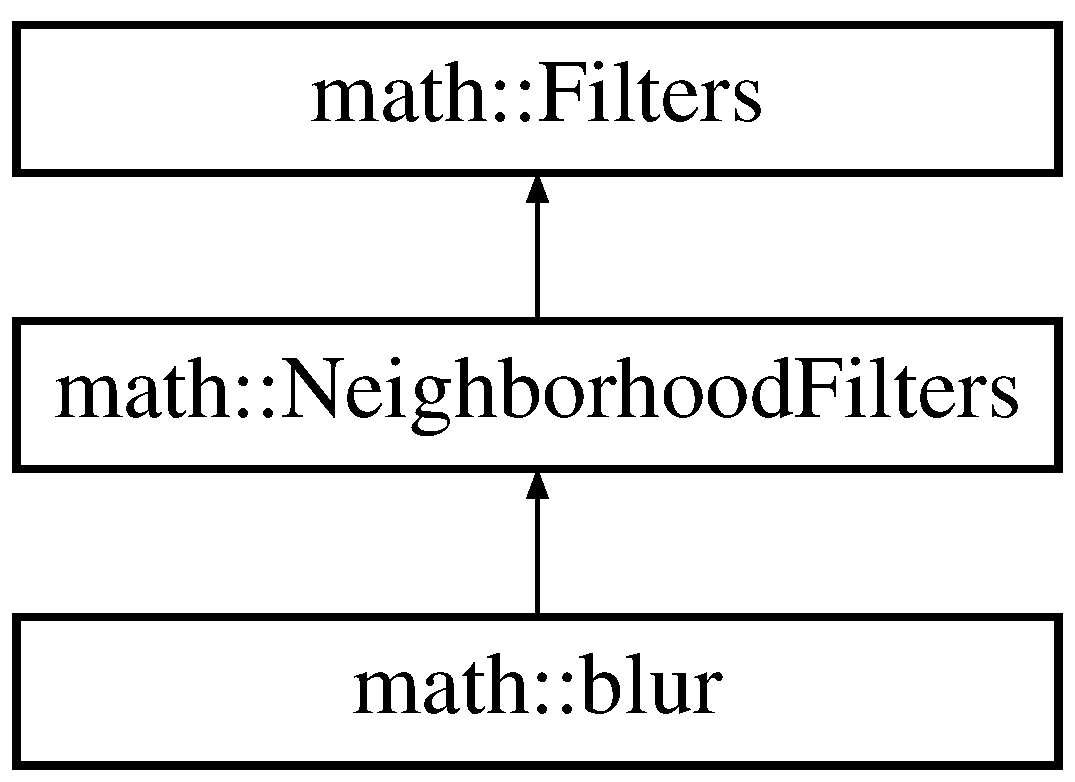
\includegraphics[height=3.000000cm]{classmath_1_1blur}
\end{center}
\end{figure}
\subsection*{Public Member Functions}
\begin{DoxyCompactItemize}
\item 
\mbox{\Hypertarget{classmath_1_1blur_a5fabbff573c2beaec676aec93945bef2}\label{classmath_1_1blur_a5fabbff573c2beaec676aec93945bef2}} 
virtual void {\bfseries filterate} (\hyperlink{classmath_1_1_image}{Image} \&sampleimage)
\end{DoxyCompactItemize}


The documentation for this class was generated from the following file\+:\begin{DoxyCompactItemize}
\item 
C\+:/\+Users/\+George/\+Documents/\+Visual Studio 2015/\+Projects/\+Team\+Project3/blur.\+h\end{DoxyCompactItemize}

\hypertarget{classmath_1_1color}{}\section{math\+:\+:color Class Reference}
\label{classmath_1_1color}\index{math\+::color@{math\+::color}}
Inheritance diagram for math\+:\+:color\+:\begin{figure}[H]
\begin{center}
\leavevmode
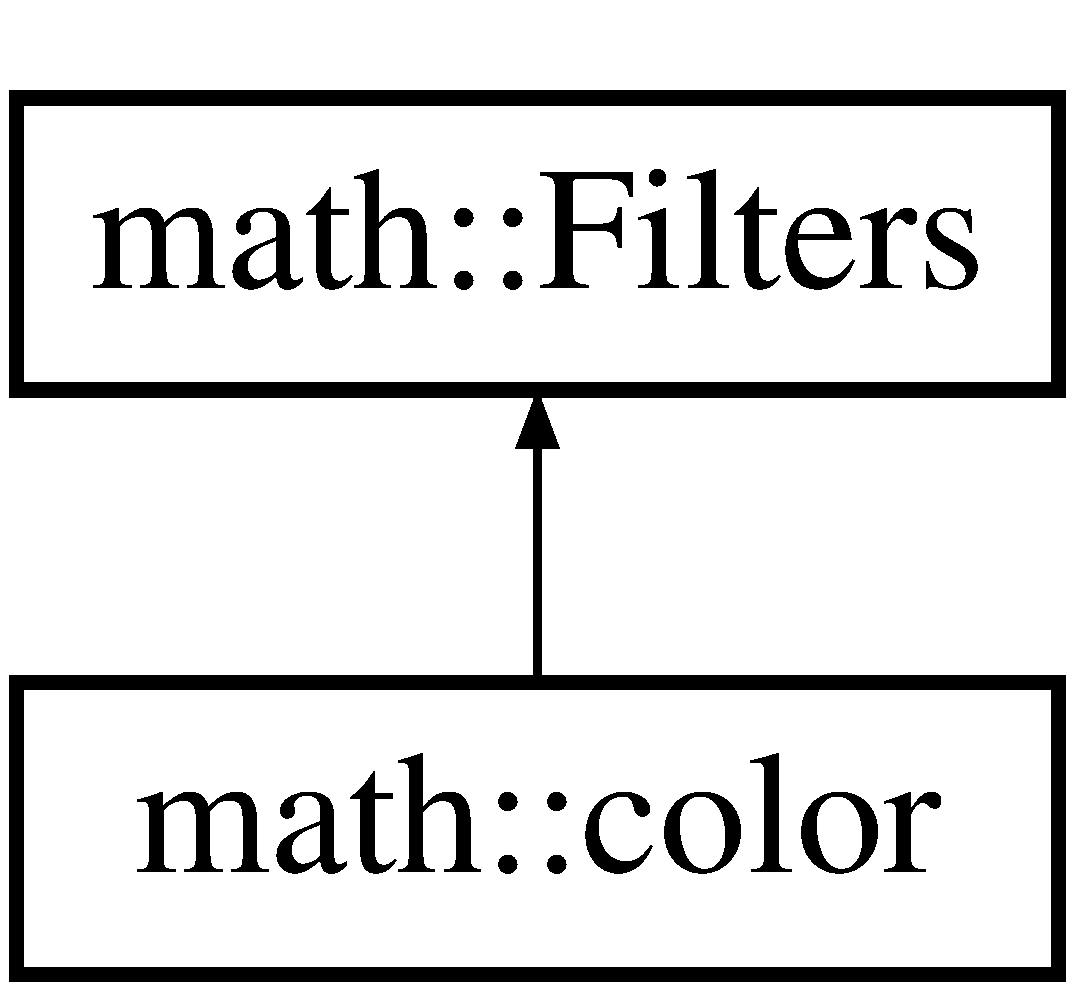
\includegraphics[height=2.000000cm]{classmath_1_1color}
\end{center}
\end{figure}
\subsection*{Public Member Functions}
\begin{DoxyCompactItemize}
\item 
\mbox{\Hypertarget{classmath_1_1color_a75daa37436356e0dc33c5d12ea955df3}\label{classmath_1_1color_a75daa37436356e0dc33c5d12ea955df3}} 
{\bfseries color\+::color} (float arg1, float arg2, float arg3)
\item 
\mbox{\Hypertarget{classmath_1_1color_a8277acf72231494e2d513267d82cb003}\label{classmath_1_1color_a8277acf72231494e2d513267d82cb003}} 
virtual void {\bfseries filterate} (\hyperlink{classmath_1_1_image}{Image} \&sampleimage)
\end{DoxyCompactItemize}


The documentation for this class was generated from the following file\+:\begin{DoxyCompactItemize}
\item 
C\+:/\+Users/\+George/\+Documents/\+Visual Studio 2015/\+Projects/\+Team\+Project3/color.\+h\end{DoxyCompactItemize}

\hypertarget{classmath_1_1diff}{}\section{math\+:\+:diff Class Reference}
\label{classmath_1_1diff}\index{math\+::diff@{math\+::diff}}
Inheritance diagram for math\+:\+:diff\+:\begin{figure}[H]
\begin{center}
\leavevmode
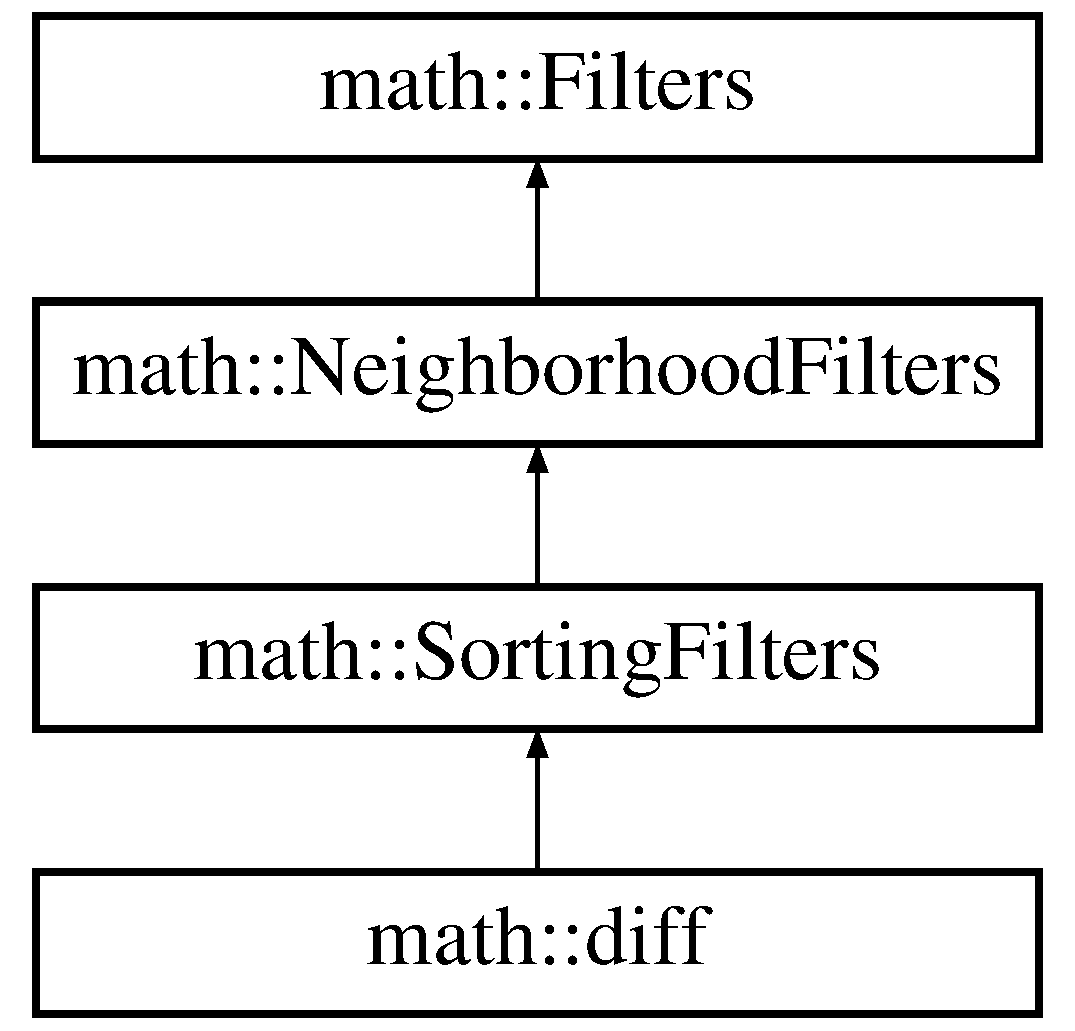
\includegraphics[height=4.000000cm]{classmath_1_1diff}
\end{center}
\end{figure}
\subsection*{Public Member Functions}
\begin{DoxyCompactItemize}
\item 
\mbox{\Hypertarget{classmath_1_1diff_a406b8ce6b7d687d05c3e2f3b639ae854}\label{classmath_1_1diff_a406b8ce6b7d687d05c3e2f3b639ae854}} 
virtual void {\bfseries filterate} (\hyperlink{classmath_1_1_image}{Image} \&sampleimage)
\end{DoxyCompactItemize}


The documentation for this class was generated from the following file\+:\begin{DoxyCompactItemize}
\item 
C\+:/\+Users/\+George/\+Documents/\+Visual Studio 2015/\+Projects/\+Team\+Project3/diff.\+h\end{DoxyCompactItemize}

\hypertarget{classmath_1_1_filters}{}\section{math\+:\+:Filters Class Reference}
\label{classmath_1_1_filters}\index{math\+::\+Filters@{math\+::\+Filters}}
Inheritance diagram for math\+:\+:Filters\+:\begin{figure}[H]
\begin{center}
\leavevmode
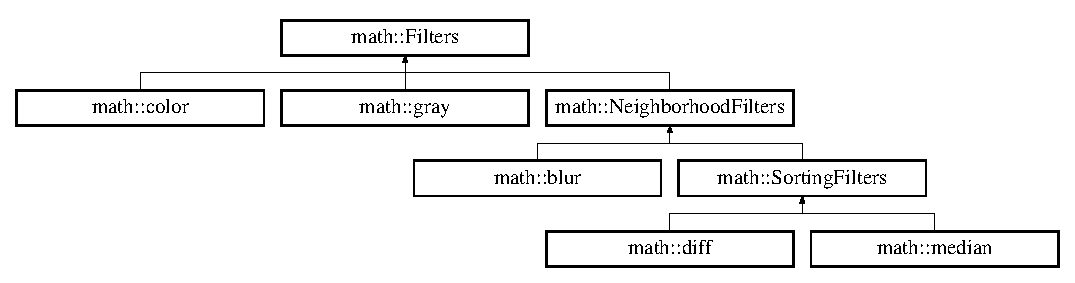
\includegraphics[height=3.353293cm]{classmath_1_1_filters}
\end{center}
\end{figure}
\subsection*{Public Member Functions}
\begin{DoxyCompactItemize}
\item 
\mbox{\Hypertarget{classmath_1_1_filters_a3c0f9f6960ec0849f74e1e91d27a93c0}\label{classmath_1_1_filters_a3c0f9f6960ec0849f74e1e91d27a93c0}} 
virtual void {\bfseries filterate} (\hyperlink{classmath_1_1_image}{Image} \&sampleimage)=0
\end{DoxyCompactItemize}


The documentation for this class was generated from the following file\+:\begin{DoxyCompactItemize}
\item 
C\+:/\+Users/\+George/\+Documents/\+Visual Studio 2015/\+Projects/\+Team\+Project3/Filters.\+h\end{DoxyCompactItemize}

\hypertarget{classmath_1_1gray}{}\section{math\+:\+:gray Class Reference}
\label{classmath_1_1gray}\index{math\+::gray@{math\+::gray}}
Inheritance diagram for math\+:\+:gray\+:\begin{figure}[H]
\begin{center}
\leavevmode
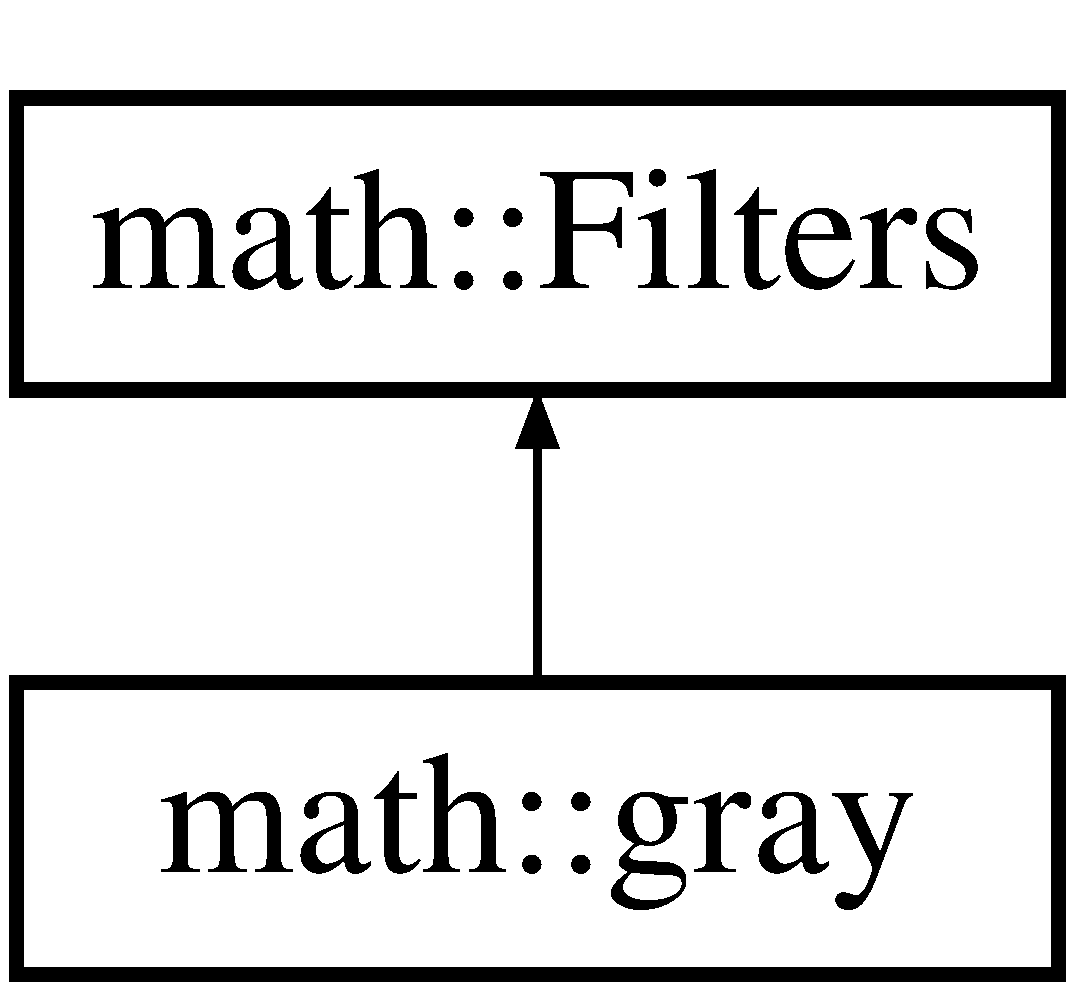
\includegraphics[height=2.000000cm]{classmath_1_1gray}
\end{center}
\end{figure}
\subsection*{Public Member Functions}
\begin{DoxyCompactItemize}
\item 
\mbox{\Hypertarget{classmath_1_1gray_aae9a8d291e2779e232d8f7231b531364}\label{classmath_1_1gray_aae9a8d291e2779e232d8f7231b531364}} 
virtual void {\bfseries filterate} (\hyperlink{classmath_1_1_image}{Image} \&sampleimage)
\end{DoxyCompactItemize}


The documentation for this class was generated from the following file\+:\begin{DoxyCompactItemize}
\item 
C\+:/\+Users/\+George/\+Documents/\+Visual Studio 2015/\+Projects/\+Team\+Project3/gray.\+h\end{DoxyCompactItemize}

\hypertarget{classmath_1_1_image}{}\section{math\+:\+:Image Class Reference}
\label{classmath_1_1_image}\index{math\+::\+Image@{math\+::\+Image}}


{\ttfamily \#include $<$Image.\+h$>$}

Inheritance diagram for math\+:\+:Image\+:\begin{figure}[H]
\begin{center}
\leavevmode
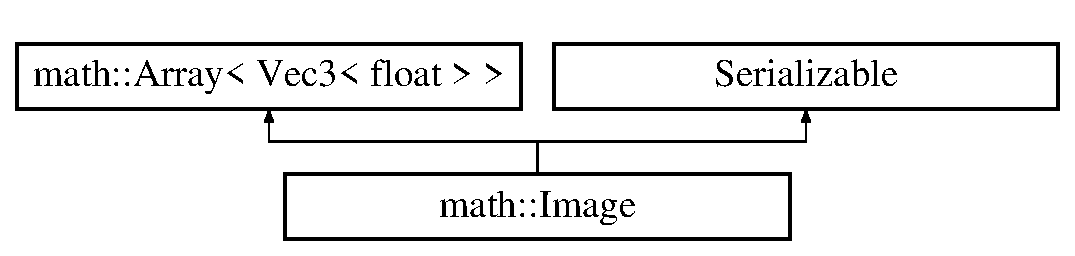
\includegraphics[height=2.000000cm]{classmath_1_1_image}
\end{center}
\end{figure}
\subsection*{Public Member Functions}
\begin{DoxyCompactItemize}
\item 
\hyperlink{classmath_1_1_vec3}{Vec3}$<$ float $>$ $\ast$ \hyperlink{classmath_1_1_image_a11850e9ecae1cced03a8ca2ad9469616}{Image\+::get\+Raw\+Data\+Ptr} ()
\item 
\hyperlink{classmath_1_1_vec3}{Vec3}$<$ float $>$ \hyperlink{classmath_1_1_image_ac3df85cc8f60c6f0b2d3de123fa9cf96}{Image\+::get\+Pixel} (unsigned int x, unsigned int y) const
\item 
void \hyperlink{classmath_1_1_image_aa2b37a157ae5f1711b7eaf15b3f6c96a}{Image\+::set\+Pixel} (unsigned int x, unsigned int y, \hyperlink{classmath_1_1_vec3}{Vec3}$<$ float $>$ \&value)
\item 
void \hyperlink{classmath_1_1_image_a6078dd91d77a6753e774466e61afd6f6}{Image\+::set\+Data} (const \hyperlink{classmath_1_1_vec3}{Vec3}$<$ float $>$ $\ast$\&data\+\_\+ptr)
\item 
void \hyperlink{classmath_1_1_image_a3dc725fbfeac02c4687bb7c7e4a184fd}{Image\+::resize} (unsigned int new\+\_\+width, unsigned int new\+\_\+height)
\item 
bool \hyperlink{classmath_1_1_image_a152102a0b98f58cd4bb6206353fb0a4f}{operator$<$$<$} (std\+::string filename)
\item 
bool \hyperlink{classmath_1_1_image_a5a48aa778e407699272463a1be8ac16f}{operator$>$$>$} (std\+::string filename)
\item 
\hyperlink{classmath_1_1_image_a845cd219c6624862cc0c632a8a9efd5f}{Image\+::\+Image} ()
\item 
\hyperlink{classmath_1_1_image_aae37c3657dd8d50277cd9eb9fa15ec7b}{Image\+::\+Image} (unsigned int \hyperlink{classmath_1_1_array_aac107e42abccdfb484b0544e6a860c10}{width}, unsigned int \hyperlink{classmath_1_1_array_a80b79625a8f11cbc63843376b591360c}{height})
\item 
\hyperlink{classmath_1_1_image_a5cccddb81385864de4c9365d3ac95596}{Image\+::\+Image} (unsigned int \hyperlink{classmath_1_1_array_aac107e42abccdfb484b0544e6a860c10}{width}, unsigned int \hyperlink{classmath_1_1_array_a80b79625a8f11cbc63843376b591360c}{height}, const \hyperlink{classmath_1_1_vec3}{Vec3}$<$ float $>$ $\ast$data\+\_\+ptr)
\item 
\hyperlink{classmath_1_1_image_ad58510b279a054e467bf6b4a78c6f75e}{Image\+::\+Image} (const \hyperlink{classmath_1_1_image}{Image} \&src)
\item 
\hyperlink{classmath_1_1_image_a584aa9f6d6f9bd80e94c773402bcf5e2}{Image\+::$\sim$\+Image} ()
\item 
\hyperlink{classmath_1_1_image}{Image} \& \hyperlink{classmath_1_1_image_a0c6305898541b826fa8f5f65333d9072}{Image\+::operator=} (const \hyperlink{classmath_1_1_image}{Image} \&right)
\end{DoxyCompactItemize}
\subsection*{Additional Inherited Members}


\subsection{Detailed Description}
It is the class that represents a generic data container for an image.

It holds the actual buffer of the pixel values and provides methods for accessing them, either as individual pixels or as a memory block. The \hyperlink{classmath_1_1_image}{Image} class alone does not provide any functionality for loading and storing an image, as it is the result or input to such a procedure.

The internal buffer of an image object stores the actual bytes (data) of the color image as a contiguous sequence of R\+GB triplets. All values stored in the internal memory buffer are floating point values and for typical (normalized) intensity ranges, each color component is within the range \mbox{[}0.\+0, 1.\+0\mbox{]}. 

\subsection{Constructor \& Destructor Documentation}
\mbox{\Hypertarget{classmath_1_1_image_a584aa9f6d6f9bd80e94c773402bcf5e2}\label{classmath_1_1_image_a584aa9f6d6f9bd80e94c773402bcf5e2}} 
\index{math\+::\+Image@{math\+::\+Image}!Image\+::$\sim$\+Image@{Image\+::$\sim$\+Image}}
\index{Image\+::$\sim$\+Image@{Image\+::$\sim$\+Image}!math\+::\+Image@{math\+::\+Image}}
\subsubsection{\texorpdfstring{Image\+::$\sim$\+Image()}{Image::~Image()}}
{\footnotesize\ttfamily math\+::\+Image\+::\+Image\+::$\sim$\+Image (\begin{DoxyParamCaption}{ }\end{DoxyParamCaption})}

The \hyperlink{classmath_1_1_image}{Image} destructor. 

\subsection{Member Function Documentation}
\mbox{\Hypertarget{classmath_1_1_image_ac3df85cc8f60c6f0b2d3de123fa9cf96}\label{classmath_1_1_image_ac3df85cc8f60c6f0b2d3de123fa9cf96}} 
\index{math\+::\+Image@{math\+::\+Image}!Image\+::get\+Pixel@{Image\+::get\+Pixel}}
\index{Image\+::get\+Pixel@{Image\+::get\+Pixel}!math\+::\+Image@{math\+::\+Image}}
\subsubsection{\texorpdfstring{Image\+::get\+Pixel()}{Image::getPixel()}}
{\footnotesize\ttfamily \hyperlink{classmath_1_1_vec3}{Vec3}$<$float$>$ math\+::\+Image\+::\+Image\+::get\+Pixel (\begin{DoxyParamCaption}\item[{unsigned int}]{x,  }\item[{unsigned int}]{y }\end{DoxyParamCaption}) const}

Obtains the color of the image at location (x,y).

The method should do any necessary bounds checking.


\begin{DoxyParams}{Parameters}
{\em x} & is the (zero-\/based) horizontal index of the pixel to get. \\
\hline
{\em y} & is the (zero-\/based) vertical index of the pixel to get.\\
\hline
\end{DoxyParams}
\begin{DoxyReturn}{Returns}
The color of the (x,y) pixel as a Color object. Returns a black (0,0,0) color in case of an out-\/of-\/bounds x,y pair. 
\end{DoxyReturn}
\mbox{\Hypertarget{classmath_1_1_image_a11850e9ecae1cced03a8ca2ad9469616}\label{classmath_1_1_image_a11850e9ecae1cced03a8ca2ad9469616}} 
\index{math\+::\+Image@{math\+::\+Image}!Image\+::get\+Raw\+Data\+Ptr@{Image\+::get\+Raw\+Data\+Ptr}}
\index{Image\+::get\+Raw\+Data\+Ptr@{Image\+::get\+Raw\+Data\+Ptr}!math\+::\+Image@{math\+::\+Image}}
\subsubsection{\texorpdfstring{Image\+::get\+Raw\+Data\+Ptr()}{Image::getRawDataPtr()}}
{\footnotesize\ttfamily \hyperlink{classmath_1_1_vec3}{Vec3}$<$float$>$$\ast$ math\+::\+Image\+::\+Image\+::get\+Raw\+Data\+Ptr (\begin{DoxyParamCaption}{ }\end{DoxyParamCaption})}

Obtains a pointer to the internal data.

This is N\+OT a copy of the internal image data, but rather a pointer to the internally allocated space, so DO N\+OT attempt to delete the pointer. \mbox{\Hypertarget{classmath_1_1_image_a845cd219c6624862cc0c632a8a9efd5f}\label{classmath_1_1_image_a845cd219c6624862cc0c632a8a9efd5f}} 
\index{math\+::\+Image@{math\+::\+Image}!Image\+::\+Image@{Image\+::\+Image}}
\index{Image\+::\+Image@{Image\+::\+Image}!math\+::\+Image@{math\+::\+Image}}
\subsubsection{\texorpdfstring{Image\+::\+Image()}{Image::Image()}\hspace{0.1cm}{\footnotesize\ttfamily [1/4]}}
{\footnotesize\ttfamily math\+::\+Image\+::\+Image\+::\+Image (\begin{DoxyParamCaption}{ }\end{DoxyParamCaption})}

Default constructor.

By default, the dimensions of the image should be zero and the buffer must be set to nullptr. \mbox{\Hypertarget{classmath_1_1_image_aae37c3657dd8d50277cd9eb9fa15ec7b}\label{classmath_1_1_image_aae37c3657dd8d50277cd9eb9fa15ec7b}} 
\index{math\+::\+Image@{math\+::\+Image}!Image\+::\+Image@{Image\+::\+Image}}
\index{Image\+::\+Image@{Image\+::\+Image}!math\+::\+Image@{math\+::\+Image}}
\subsubsection{\texorpdfstring{Image\+::\+Image()}{Image::Image()}\hspace{0.1cm}{\footnotesize\ttfamily [2/4]}}
{\footnotesize\ttfamily math\+::\+Image\+::\+Image\+::\+Image (\begin{DoxyParamCaption}\item[{unsigned int}]{width,  }\item[{unsigned int}]{height }\end{DoxyParamCaption})}

Constructor with width and height specification.


\begin{DoxyParams}{Parameters}
{\em width} & is the desired width of the new image. \\
\hline
{\em height} & is the desired height of the new image. \\
\hline
\end{DoxyParams}
\mbox{\Hypertarget{classmath_1_1_image_a5cccddb81385864de4c9365d3ac95596}\label{classmath_1_1_image_a5cccddb81385864de4c9365d3ac95596}} 
\index{math\+::\+Image@{math\+::\+Image}!Image\+::\+Image@{Image\+::\+Image}}
\index{Image\+::\+Image@{Image\+::\+Image}!math\+::\+Image@{math\+::\+Image}}
\subsubsection{\texorpdfstring{Image\+::\+Image()}{Image::Image()}\hspace{0.1cm}{\footnotesize\ttfamily [3/4]}}
{\footnotesize\ttfamily math\+::\+Image\+::\+Image\+::\+Image (\begin{DoxyParamCaption}\item[{unsigned int}]{width,  }\item[{unsigned int}]{height,  }\item[{const \hyperlink{classmath_1_1_vec3}{Vec3}$<$ float $>$ $\ast$}]{data\+\_\+ptr }\end{DoxyParamCaption})}

Constructor with data initialization.


\begin{DoxyParams}{Parameters}
{\em width} & is the desired width of the new image. \\
\hline
{\em height} & is the desired height of the new image. \\
\hline
{\em data\+\_\+ptr} & is the source of the data to copy to the internal image buffer.\\
\hline
\end{DoxyParams}
\begin{DoxySeeAlso}{See also}
set\+Data 
\end{DoxySeeAlso}
\mbox{\Hypertarget{classmath_1_1_image_ad58510b279a054e467bf6b4a78c6f75e}\label{classmath_1_1_image_ad58510b279a054e467bf6b4a78c6f75e}} 
\index{math\+::\+Image@{math\+::\+Image}!Image\+::\+Image@{Image\+::\+Image}}
\index{Image\+::\+Image@{Image\+::\+Image}!math\+::\+Image@{math\+::\+Image}}
\subsubsection{\texorpdfstring{Image\+::\+Image()}{Image::Image()}\hspace{0.1cm}{\footnotesize\ttfamily [4/4]}}
{\footnotesize\ttfamily math\+::\+Image\+::\+Image\+::\+Image (\begin{DoxyParamCaption}\item[{const \hyperlink{classmath_1_1_image}{Image} \&}]{src }\end{DoxyParamCaption})}

Copy constructor.


\begin{DoxyParams}{Parameters}
{\em src} & is the source image to replicate in this object. \\
\hline
\end{DoxyParams}
\mbox{\Hypertarget{classmath_1_1_image_a0c6305898541b826fa8f5f65333d9072}\label{classmath_1_1_image_a0c6305898541b826fa8f5f65333d9072}} 
\index{math\+::\+Image@{math\+::\+Image}!Image\+::operator=@{Image\+::operator=}}
\index{Image\+::operator=@{Image\+::operator=}!math\+::\+Image@{math\+::\+Image}}
\subsubsection{\texorpdfstring{Image\+::operator=()}{Image::operator=()}}
{\footnotesize\ttfamily \hyperlink{classmath_1_1_image}{Image}\& math\+::\+Image\+::\+Image\+::operator= (\begin{DoxyParamCaption}\item[{const \hyperlink{classmath_1_1_image}{Image} \&}]{right }\end{DoxyParamCaption})}

Copy assignment operator.


\begin{DoxyParams}{Parameters}
{\em right} & is the source image. \\
\hline
\end{DoxyParams}
\mbox{\Hypertarget{classmath_1_1_image_a3dc725fbfeac02c4687bb7c7e4a184fd}\label{classmath_1_1_image_a3dc725fbfeac02c4687bb7c7e4a184fd}} 
\index{math\+::\+Image@{math\+::\+Image}!Image\+::resize@{Image\+::resize}}
\index{Image\+::resize@{Image\+::resize}!math\+::\+Image@{math\+::\+Image}}
\subsubsection{\texorpdfstring{Image\+::resize()}{Image::resize()}}
{\footnotesize\ttfamily void math\+::\+Image\+::\+Image\+::resize (\begin{DoxyParamCaption}\item[{unsigned int}]{new\+\_\+width,  }\item[{unsigned int}]{new\+\_\+height }\end{DoxyParamCaption})}

Changes the internal image data storage size.

If the one or both of the given dimensions are smaller, the image should be clipped by discarding the remaining pixels in the rows and/or columns outside the margins. If the new dimensions are larger, pad the old pixels with zero values (black color). If the image is not yet allocated (zero width and height), allocate the internal buffer and set the image size according to the given dimensions.


\begin{DoxyParams}{Parameters}
{\em new\+\_\+width} & is the user-\/provided width to resize the image storage to. \\
\hline
{\em new\+\_\+height} & is the user-\/provided height to resize the image storage to. \\
\hline
\end{DoxyParams}
\mbox{\Hypertarget{classmath_1_1_image_a6078dd91d77a6753e774466e61afd6f6}\label{classmath_1_1_image_a6078dd91d77a6753e774466e61afd6f6}} 
\index{math\+::\+Image@{math\+::\+Image}!Image\+::set\+Data@{Image\+::set\+Data}}
\index{Image\+::set\+Data@{Image\+::set\+Data}!math\+::\+Image@{math\+::\+Image}}
\subsubsection{\texorpdfstring{Image\+::set\+Data()}{Image::setData()}}
{\footnotesize\ttfamily void math\+::\+Image\+::\+Image\+::set\+Data (\begin{DoxyParamCaption}\item[{const \hyperlink{classmath_1_1_vec3}{Vec3}$<$ float $>$ $\ast$\&}]{data\+\_\+ptr }\end{DoxyParamCaption})}

Copies the image data from an external raw buffer to the internal image buffer.

The member function A\+S\+S\+U\+M\+ES that the input buffer is of a size compatible with the internal storage of the \hyperlink{classmath_1_1_image}{Image} object and that the data buffer has been alreeady allocated. If the image buffer is not allocated or the width or height of the image are 0, the method should exit immediately.


\begin{DoxyParams}{Parameters}
{\em data\+\_\+ptr} & is the reference to the preallocated buffer from where to copy the data to the \hyperlink{classmath_1_1_image}{Image} object. \\
\hline
\end{DoxyParams}
\mbox{\Hypertarget{classmath_1_1_image_aa2b37a157ae5f1711b7eaf15b3f6c96a}\label{classmath_1_1_image_aa2b37a157ae5f1711b7eaf15b3f6c96a}} 
\index{math\+::\+Image@{math\+::\+Image}!Image\+::set\+Pixel@{Image\+::set\+Pixel}}
\index{Image\+::set\+Pixel@{Image\+::set\+Pixel}!math\+::\+Image@{math\+::\+Image}}
\subsubsection{\texorpdfstring{Image\+::set\+Pixel()}{Image::setPixel()}}
{\footnotesize\ttfamily void math\+::\+Image\+::\+Image\+::set\+Pixel (\begin{DoxyParamCaption}\item[{unsigned int}]{x,  }\item[{unsigned int}]{y,  }\item[{\hyperlink{classmath_1_1_vec3}{Vec3}$<$ float $>$ \&}]{value }\end{DoxyParamCaption})}

Sets the R\+GB values for an (x,y) pixel.

The method should perform any necessary bounds checking.


\begin{DoxyParams}{Parameters}
{\em x} & is the (zero-\/based) horizontal index of the pixel to set. \\
\hline
{\em y} & is the (zero-\/based) vertical index of the pixel to set. \\
\hline
{\em value} & is the new color for the (x,y) pixel. \\
\hline
\end{DoxyParams}
\mbox{\Hypertarget{classmath_1_1_image_a152102a0b98f58cd4bb6206353fb0a4f}\label{classmath_1_1_image_a152102a0b98f58cd4bb6206353fb0a4f}} 
\index{math\+::\+Image@{math\+::\+Image}!operator$<$$<$@{operator$<$$<$}}
\index{operator$<$$<$@{operator$<$$<$}!math\+::\+Image@{math\+::\+Image}}
\subsubsection{\texorpdfstring{operator$<$$<$()}{operator<<()}}
{\footnotesize\ttfamily bool math\+::\+Image\+::operator$<$$<$ (\begin{DoxyParamCaption}\item[{std\+::string}]{filename }\end{DoxyParamCaption})\hspace{0.3cm}{\ttfamily [virtual]}}

Reads the contents of an object from the specified file.

The operator can be used for the implementation of \char`\"{}de-\/serialization\char`\"{}.


\begin{DoxyParams}{Parameters}
{\em filename} & is the name of the file to use for loading the data.\\
\hline
\end{DoxyParams}
\begin{DoxyReturn}{Returns}
true if the operation was successful, false otherwise. 
\end{DoxyReturn}


Implements \hyperlink{class_serializable_a5a8ec3fd8411693715ac76b1a10386ba}{Serializable}.

\mbox{\Hypertarget{classmath_1_1_image_a5a48aa778e407699272463a1be8ac16f}\label{classmath_1_1_image_a5a48aa778e407699272463a1be8ac16f}} 
\index{math\+::\+Image@{math\+::\+Image}!operator$>$$>$@{operator$>$$>$}}
\index{operator$>$$>$@{operator$>$$>$}!math\+::\+Image@{math\+::\+Image}}
\subsubsection{\texorpdfstring{operator$>$$>$()}{operator>>()}}
{\footnotesize\ttfamily bool math\+::\+Image\+::operator$>$$>$ (\begin{DoxyParamCaption}\item[{std\+::string}]{filename }\end{DoxyParamCaption})\hspace{0.3cm}{\ttfamily [virtual]}}

Writes the contents of an object to the specified file.

The operator can be used for the implementation of \char`\"{}serialization\char`\"{}.


\begin{DoxyParams}{Parameters}
{\em filename} & is the name of the file to use for saving the data.\\
\hline
\end{DoxyParams}
\begin{DoxyReturn}{Returns}
true if the operation was successful, false otherwise. 
\end{DoxyReturn}


Implements \hyperlink{class_serializable_a60c53d8ec7e38531699d1ca19642318d}{Serializable}.



The documentation for this class was generated from the following files\+:\begin{DoxyCompactItemize}
\item 
C\+:/\+Users/\+George/\+Documents/\+Visual Studio 2015/\+Projects/\+Team\+Project3/Image.\+h\item 
C\+:/\+Users/\+George/\+Documents/\+Visual Studio 2015/\+Projects/\+Team\+Project3/Image.\+cpp\end{DoxyCompactItemize}

\hypertarget{classmath_1_1median}{}\section{math\+:\+:median Class Reference}
\label{classmath_1_1median}\index{math\+::median@{math\+::median}}
Inheritance diagram for math\+:\+:median\+:\begin{figure}[H]
\begin{center}
\leavevmode
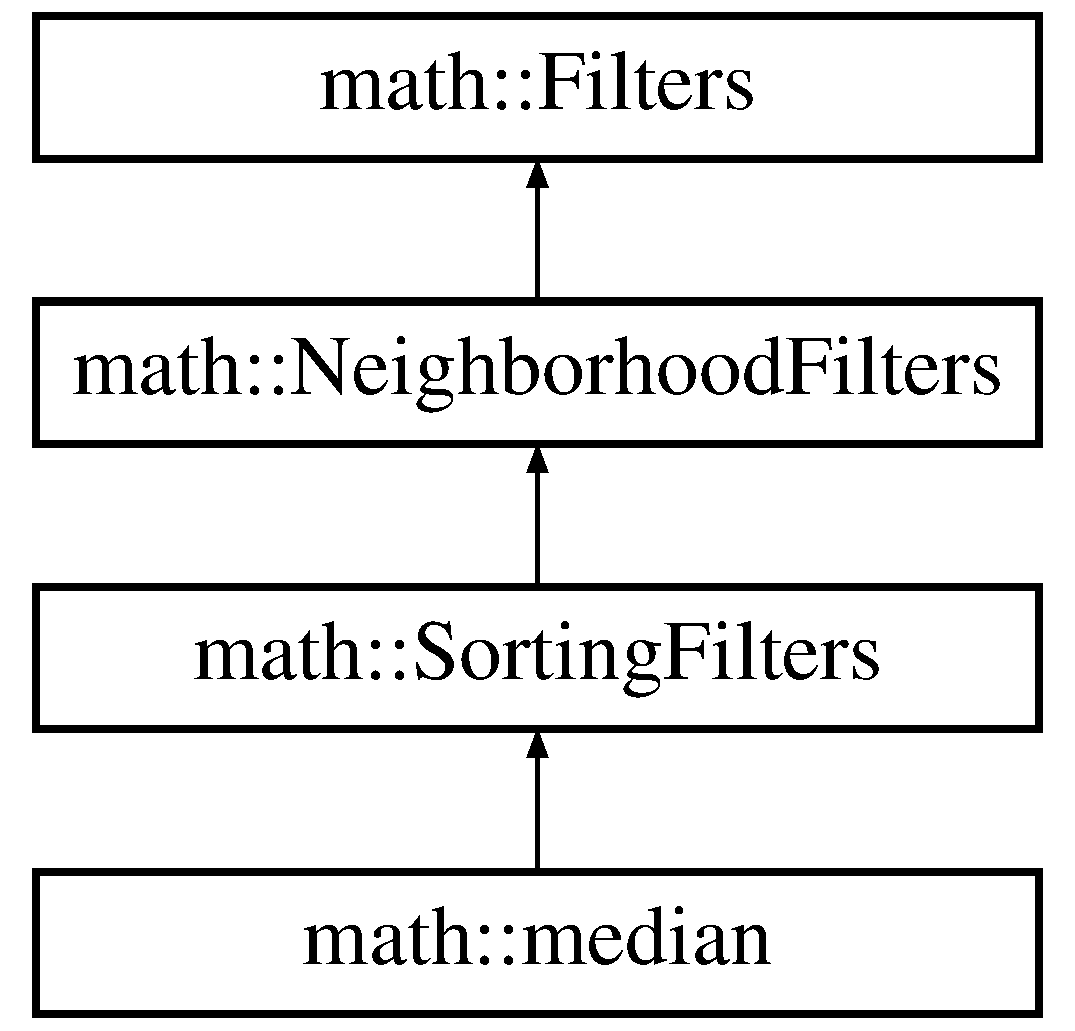
\includegraphics[height=4.000000cm]{classmath_1_1median}
\end{center}
\end{figure}
\subsection*{Public Member Functions}
\begin{DoxyCompactItemize}
\item 
\mbox{\Hypertarget{classmath_1_1median_ab7aee9bfb443bee0bb6766c07978372b}\label{classmath_1_1median_ab7aee9bfb443bee0bb6766c07978372b}} 
virtual void {\bfseries filterate} (\hyperlink{classmath_1_1_image}{Image} \&sampleimage)
\end{DoxyCompactItemize}


The documentation for this class was generated from the following file\+:\begin{DoxyCompactItemize}
\item 
C\+:/\+Users/\+George/\+Documents/\+Visual Studio 2015/\+Projects/\+Team\+Project3/median.\+h\end{DoxyCompactItemize}

\hypertarget{classmath_1_1_neighborhood_filters}{}\section{math\+:\+:Neighborhood\+Filters Class Reference}
\label{classmath_1_1_neighborhood_filters}\index{math\+::\+Neighborhood\+Filters@{math\+::\+Neighborhood\+Filters}}
Inheritance diagram for math\+:\+:Neighborhood\+Filters\+:\begin{figure}[H]
\begin{center}
\leavevmode
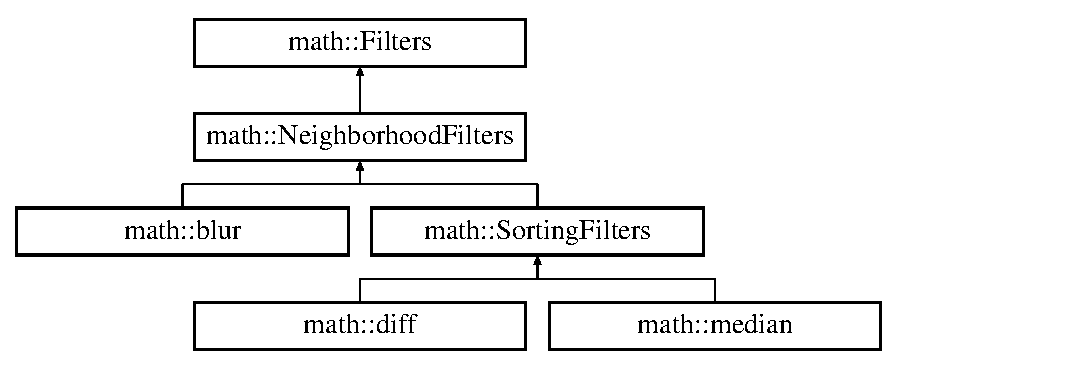
\includegraphics[height=4.000000cm]{classmath_1_1_neighborhood_filters}
\end{center}
\end{figure}
\subsection*{Public Member Functions}
\begin{DoxyCompactItemize}
\item 
\mbox{\Hypertarget{classmath_1_1_neighborhood_filters_a6a3e440fd09b3481a74f81de9627d3a2}\label{classmath_1_1_neighborhood_filters_a6a3e440fd09b3481a74f81de9627d3a2}} 
virtual void {\bfseries filterate} (\hyperlink{classmath_1_1_image}{Image} \&sampleimage)=0
\item 
\mbox{\Hypertarget{classmath_1_1_neighborhood_filters_afe9f90299c1a6ff6ff758f03fa3c8931}\label{classmath_1_1_neighborhood_filters_afe9f90299c1a6ff6ff758f03fa3c8931}} 
virtual bool {\bfseries check\+If\+Valid} (\hyperlink{classmath_1_1_image}{Image} \&sampleimage, size\+\_\+t x, size\+\_\+t y)
\end{DoxyCompactItemize}


The documentation for this class was generated from the following file\+:\begin{DoxyCompactItemize}
\item 
C\+:/\+Users/\+George/\+Documents/\+Visual Studio 2015/\+Projects/\+Team\+Project3/Neighborhood\+Filters.\+h\end{DoxyCompactItemize}

\hypertarget{class_serializable}{}\section{Serializable Class Reference}
\label{class_serializable}\index{Serializable@{Serializable}}


{\ttfamily \#include $<$Serializable.\+h$>$}

Inheritance diagram for Serializable\+:\begin{figure}[H]
\begin{center}
\leavevmode
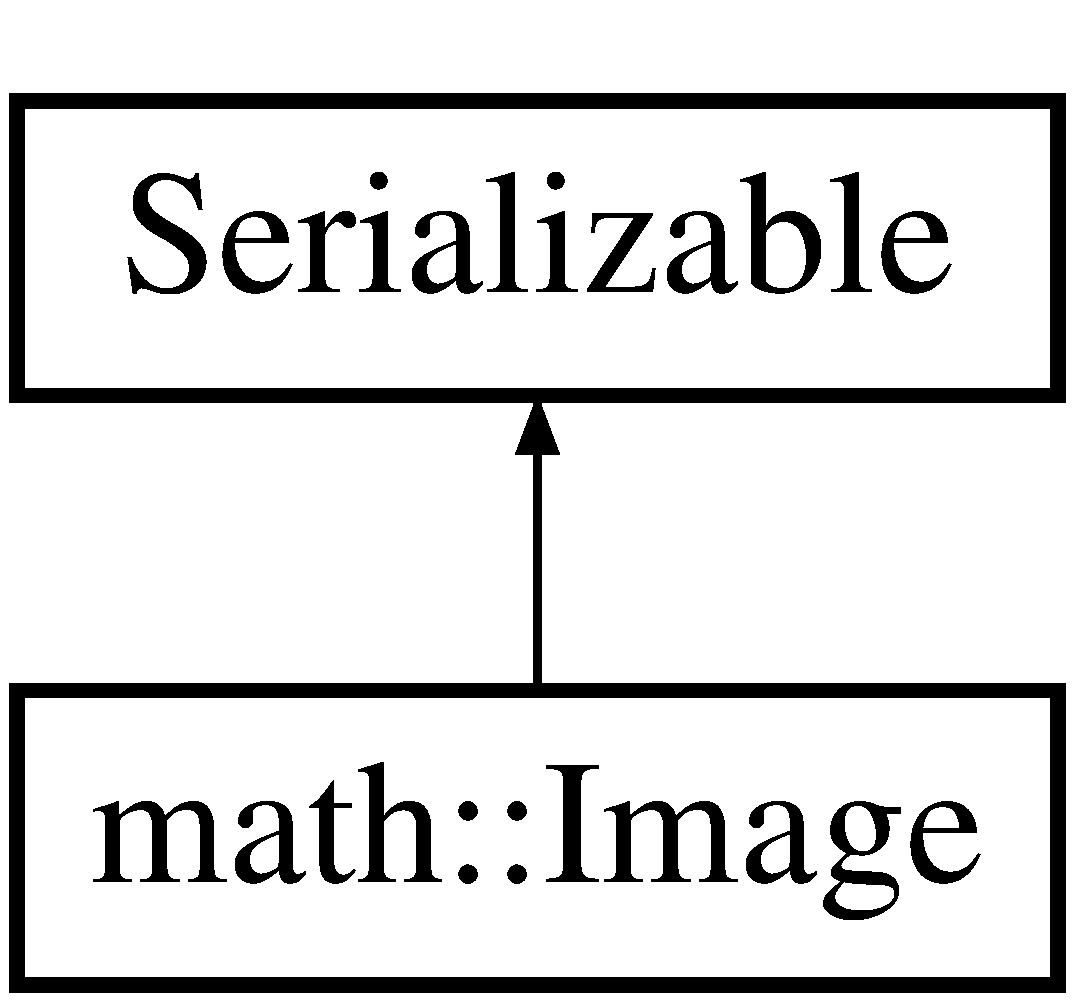
\includegraphics[height=2.000000cm]{class_serializable}
\end{center}
\end{figure}
\subsection*{Public Member Functions}
\begin{DoxyCompactItemize}
\item 
virtual bool \hyperlink{class_serializable_a5a8ec3fd8411693715ac76b1a10386ba}{operator$<$$<$} (std\+::string filename)=0
\item 
virtual bool \hyperlink{class_serializable_a60c53d8ec7e38531699d1ca19642318d}{operator$>$$>$} (std\+::string filename)=0
\end{DoxyCompactItemize}


\subsection{Detailed Description}
Interface for object serialization to a file.

Provides two operators that objects derived from this class can use to store and load their data from a file, Using a custom implementation for them. 

\subsection{Member Function Documentation}
\mbox{\Hypertarget{class_serializable_a5a8ec3fd8411693715ac76b1a10386ba}\label{class_serializable_a5a8ec3fd8411693715ac76b1a10386ba}} 
\index{Serializable@{Serializable}!operator$<$$<$@{operator$<$$<$}}
\index{operator$<$$<$@{operator$<$$<$}!Serializable@{Serializable}}
\subsubsection{\texorpdfstring{operator$<$$<$()}{operator<<()}}
{\footnotesize\ttfamily virtual bool Serializable\+::operator$<$$<$ (\begin{DoxyParamCaption}\item[{std\+::string}]{filename }\end{DoxyParamCaption})\hspace{0.3cm}{\ttfamily [pure virtual]}}

Reads the contents of an object from the specified file.

The operator can be used for the implementation of \char`\"{}de-\/serialization\char`\"{}.


\begin{DoxyParams}{Parameters}
{\em filename} & is the name of the file to use for loading the data.\\
\hline
\end{DoxyParams}
\begin{DoxyReturn}{Returns}
true if the operation was successful, false otherwise. 
\end{DoxyReturn}


Implemented in \hyperlink{classmath_1_1_image_a152102a0b98f58cd4bb6206353fb0a4f}{math\+::\+Image}.

\mbox{\Hypertarget{class_serializable_a60c53d8ec7e38531699d1ca19642318d}\label{class_serializable_a60c53d8ec7e38531699d1ca19642318d}} 
\index{Serializable@{Serializable}!operator$>$$>$@{operator$>$$>$}}
\index{operator$>$$>$@{operator$>$$>$}!Serializable@{Serializable}}
\subsubsection{\texorpdfstring{operator$>$$>$()}{operator>>()}}
{\footnotesize\ttfamily virtual bool Serializable\+::operator$>$$>$ (\begin{DoxyParamCaption}\item[{std\+::string}]{filename }\end{DoxyParamCaption})\hspace{0.3cm}{\ttfamily [pure virtual]}}

Writes the contents of an object to the specified file.

The operator can be used for the implementation of \char`\"{}serialization\char`\"{}.


\begin{DoxyParams}{Parameters}
{\em filename} & is the name of the file to use for saving the data.\\
\hline
\end{DoxyParams}
\begin{DoxyReturn}{Returns}
true if the operation was successful, false otherwise. 
\end{DoxyReturn}


Implemented in \hyperlink{classmath_1_1_image_a5a48aa778e407699272463a1be8ac16f}{math\+::\+Image}.



The documentation for this class was generated from the following file\+:\begin{DoxyCompactItemize}
\item 
C\+:/\+Users/\+George/\+Documents/\+Visual Studio 2015/\+Projects/\+Team\+Project3/Serializable.\+h\end{DoxyCompactItemize}

\hypertarget{classmath_1_1_sorting_filters}{}\section{math\+:\+:Sorting\+Filters Class Reference}
\label{classmath_1_1_sorting_filters}\index{math\+::\+Sorting\+Filters@{math\+::\+Sorting\+Filters}}
Inheritance diagram for math\+:\+:Sorting\+Filters\+:\begin{figure}[H]
\begin{center}
\leavevmode
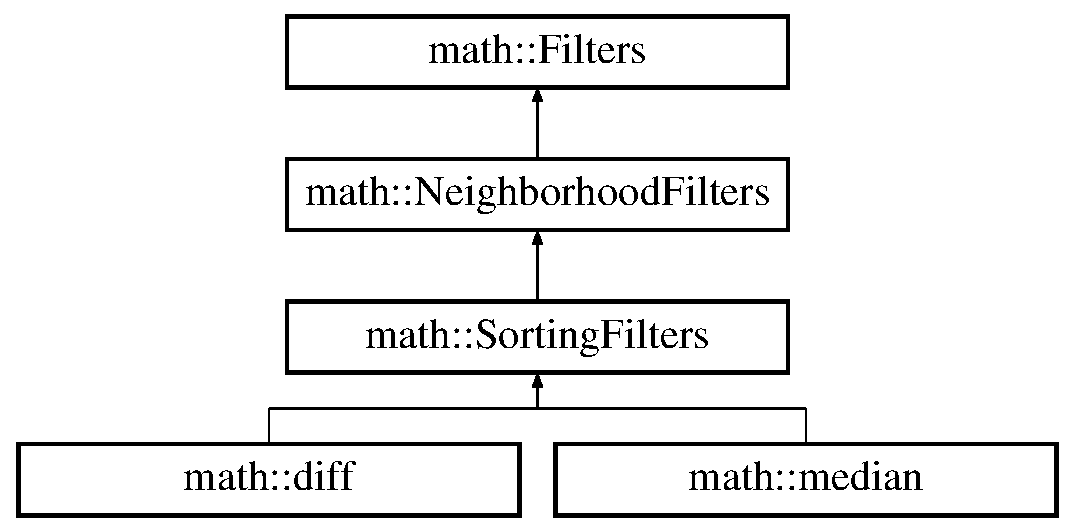
\includegraphics[height=4.000000cm]{classmath_1_1_sorting_filters}
\end{center}
\end{figure}
\subsection*{Public Member Functions}
\begin{DoxyCompactItemize}
\item 
\mbox{\Hypertarget{classmath_1_1_sorting_filters_a50faab9426081c8c685b885e71266963}\label{classmath_1_1_sorting_filters_a50faab9426081c8c685b885e71266963}} 
virtual void {\bfseries filterate} (\hyperlink{classmath_1_1_image}{Image} \&sampleimage)=0
\item 
\mbox{\Hypertarget{classmath_1_1_sorting_filters_a102e6a36d0d0ed2505723ed97b0da1d6}\label{classmath_1_1_sorting_filters_a102e6a36d0d0ed2505723ed97b0da1d6}} 
virtual void {\bfseries bubble\+Sort} (float $\ast$pixelarray, size\+\_\+t arraysize)
\end{DoxyCompactItemize}


The documentation for this class was generated from the following file\+:\begin{DoxyCompactItemize}
\item 
C\+:/\+Users/\+George/\+Documents/\+Visual Studio 2015/\+Projects/\+Team\+Project3/Sorting\+Filters.\+h\end{DoxyCompactItemize}

\hypertarget{classmath_1_1_vec3}{}\section{math\+:\+:Vec3$<$ S $>$ Class Template Reference}
\label{classmath_1_1_vec3}\index{math\+::\+Vec3$<$ S $>$@{math\+::\+Vec3$<$ S $>$}}


{\ttfamily \#include $<$Vec3.\+h$>$}

\subsection*{Public Member Functions}
\begin{DoxyCompactItemize}
\item 
S \& \hyperlink{classmath_1_1_vec3_a1748c205116e0af40aa83f2b6779e793}{operator\mbox{[}$\,$\mbox{]}} (size\+\_\+t index)
\item 
\hyperlink{classmath_1_1_vec3}{Vec3}$<$ S $>$ \hyperlink{classmath_1_1_vec3_a4b0af91c5c4825772e20568d3a132c2d}{operator+} (const \hyperlink{classmath_1_1_vec3}{Vec3}$<$ S $>$ \&right)
\item 
\hyperlink{classmath_1_1_vec3}{Vec3}$<$ S $>$ \hyperlink{classmath_1_1_vec3_a0a0ac5cc4b2e39cf68adc28442747651}{operator-\/} (const \hyperlink{classmath_1_1_vec3}{Vec3}$<$ S $>$ \&right)
\item 
\hyperlink{classmath_1_1_vec3}{Vec3}$<$ S $>$ \hyperlink{classmath_1_1_vec3_aeafba08a1b074a3fc550c76b85e15f1b}{operator$\ast$} (const \hyperlink{classmath_1_1_vec3}{Vec3}$<$ S $>$ \&right)
\item 
\hyperlink{classmath_1_1_vec3}{Vec3}$<$ S $>$ \hyperlink{classmath_1_1_vec3_a0b6b8e5f817bb76537452b0df7fbdd06}{operator$\ast$} (S right)
\item 
\hyperlink{classmath_1_1_vec3}{Vec3}$<$ S $>$ \hyperlink{classmath_1_1_vec3_aeac6cb88e12f56a13f086a1cecfae1c1}{operator/} (S right)
\item 
\hyperlink{classmath_1_1_vec3}{Vec3}$<$ S $>$ \hyperlink{classmath_1_1_vec3_a146b07bcbe24f5a380276adb8270b10e}{operator/} (const \hyperlink{classmath_1_1_vec3}{Vec3}$<$ S $>$ \&right)
\item 
\hyperlink{classmath_1_1_vec3}{Vec3}$<$ S $>$ \& \hyperlink{classmath_1_1_vec3_abd59720702df202ce59c5d5de5901f4b}{operator+=} (const \hyperlink{classmath_1_1_vec3}{Vec3}$<$ S $>$ \&right)
\item 
\hyperlink{classmath_1_1_vec3}{Vec3}$<$ S $>$ \& \hyperlink{classmath_1_1_vec3_a8e49dbf07da4a23576e7b76d3465279d}{operator-\/=} (const \hyperlink{classmath_1_1_vec3}{Vec3}$<$ S $>$ \&right)
\item 
\hyperlink{classmath_1_1_vec3}{Vec3}$<$ S $>$ \& \hyperlink{classmath_1_1_vec3_a870bc06ba74c497da633b3801ebaea0d}{operator/=} (const \hyperlink{classmath_1_1_vec3}{Vec3}$<$ S $>$ \&right)
\item 
\hyperlink{classmath_1_1_vec3}{Vec3}$<$ S $>$ \& \hyperlink{classmath_1_1_vec3_a849a0602d155721bd4ab79edc83c5e57}{operator$\ast$=} (const \hyperlink{classmath_1_1_vec3}{Vec3}$<$ S $>$ \&right)
\item 
\hyperlink{classmath_1_1_vec3}{Vec3}$<$ S $>$ \& \hyperlink{classmath_1_1_vec3_af54d3d2a6b077d8b70a8b1b71d9f6212}{operator$\ast$=} (S right)
\item 
\hyperlink{classmath_1_1_vec3}{Vec3}$<$ S $>$ \& \hyperlink{classmath_1_1_vec3_af25a74b600edcac72bc64c6316ea3252}{operator/=} (S right)
\item 
\hyperlink{classmath_1_1_vec3_a1acc8b1b1c73c5a3d1f0c60e8e23eba3}{Vec3} (S x, S y, S z)
\item 
\hyperlink{classmath_1_1_vec3_ab09aedfee5f79e9b556cc7dca8d5d011}{Vec3} (S val)
\item 
\hyperlink{classmath_1_1_vec3_a0eaf2f3a472502f1374a7f1118d7e459}{Vec3} ()
\item 
\hyperlink{classmath_1_1_vec3_a02c4f66911fc141e48d521a9a6cd9de4}{Vec3} (const \hyperlink{classmath_1_1_vec3}{Vec3}$<$ S $>$ \&right)
\item 
\hyperlink{classmath_1_1_vec3}{Vec3}$<$ S $>$ \& \hyperlink{classmath_1_1_vec3_abcc60135e1b3f3c66e89d502f5895f41}{operator=} (const \hyperlink{classmath_1_1_vec3}{Vec3}$<$ S $>$ \&right)
\item 
bool \hyperlink{classmath_1_1_vec3_a7d6020565ceec5656b4d5880c8a79a65}{operator==} (const \hyperlink{classmath_1_1_vec3}{Vec3}$<$ S $>$ \&right) const
\item 
bool \hyperlink{classmath_1_1_vec3_a98bca9bbb2161b89cf657bb6f7ae0699}{operator!=} (const \hyperlink{classmath_1_1_vec3}{Vec3}$<$ S $>$ \&right) const
\end{DoxyCompactItemize}
\subsection*{Public Attributes}
\begin{DoxyCompactItemize}
\item 
\mbox{\Hypertarget{classmath_1_1_vec3_a540f559cb87f94bfa8b61dbdfa9926c0}\label{classmath_1_1_vec3_a540f559cb87f94bfa8b61dbdfa9926c0}} 
\begin{tabbing}
xx\=xx\=xx\=xx\=xx\=xx\=xx\=xx\=xx\=\kill
union \{\\
\>S {\bfseries x}\\
\>S {\bfseries r}\\
\}; \\

\end{tabbing}\begin{DoxyCompactList}\small\item\em The first coordinate of the vector. \end{DoxyCompactList}\item 
\mbox{\Hypertarget{classmath_1_1_vec3_aceb46a7ac1d3efd1e48179bd823dc298}\label{classmath_1_1_vec3_aceb46a7ac1d3efd1e48179bd823dc298}} 
\begin{tabbing}
xx\=xx\=xx\=xx\=xx\=xx\=xx\=xx\=xx\=\kill
union \{\\
\>S {\bfseries y}\\
\>S {\bfseries g}\\
\}; \\

\end{tabbing}\begin{DoxyCompactList}\small\item\em The second coordinate of the vector. \end{DoxyCompactList}\item 
\mbox{\Hypertarget{classmath_1_1_vec3_a6c67c986fe777e5dd85a432e46487858}\label{classmath_1_1_vec3_a6c67c986fe777e5dd85a432e46487858}} 
\begin{tabbing}
xx\=xx\=xx\=xx\=xx\=xx\=xx\=xx\=xx\=\kill
union \{\\
\>S {\bfseries z}\\
\>S {\bfseries b}\\
\}; \\

\end{tabbing}\begin{DoxyCompactList}\small\item\em The third coordinate of the vector. \end{DoxyCompactList}\end{DoxyCompactItemize}


\subsection{Detailed Description}
\subsubsection*{template$<$typename S$>$\newline
class math\+::\+Vec3$<$ S $>$}

Represents a triplet of values of the same type S.

The \hyperlink{classmath_1_1_vec3}{Vec3} class is used as a generic three-\/dimensional vector and thus it defines several numerical operators that can be used on Vec3$<$\+S$>$ and S data. 

\subsection{Constructor \& Destructor Documentation}
\mbox{\Hypertarget{classmath_1_1_vec3_a1acc8b1b1c73c5a3d1f0c60e8e23eba3}\label{classmath_1_1_vec3_a1acc8b1b1c73c5a3d1f0c60e8e23eba3}} 
\index{math\+::\+Vec3@{math\+::\+Vec3}!Vec3@{Vec3}}
\index{Vec3@{Vec3}!math\+::\+Vec3@{math\+::\+Vec3}}
\subsubsection{\texorpdfstring{Vec3()}{Vec3()}\hspace{0.1cm}{\footnotesize\ttfamily [1/4]}}
{\footnotesize\ttfamily template$<$typename S$>$ \\
\hyperlink{classmath_1_1_vec3}{math\+::\+Vec3}$<$ S $>$\+::\hyperlink{classmath_1_1_vec3}{Vec3} (\begin{DoxyParamCaption}\item[{S}]{x,  }\item[{S}]{y,  }\item[{S}]{z }\end{DoxyParamCaption})\hspace{0.3cm}{\ttfamily [inline]}}

Constructor with three-\/element initialization.


\begin{DoxyParams}{Parameters}
{\em x} & is the value of th first element. \\
\hline
{\em y} & is the value of the second element. \\
\hline
{\em z} & is the value of the third element. \\
\hline
\end{DoxyParams}
\mbox{\Hypertarget{classmath_1_1_vec3_ab09aedfee5f79e9b556cc7dca8d5d011}\label{classmath_1_1_vec3_ab09aedfee5f79e9b556cc7dca8d5d011}} 
\index{math\+::\+Vec3@{math\+::\+Vec3}!Vec3@{Vec3}}
\index{Vec3@{Vec3}!math\+::\+Vec3@{math\+::\+Vec3}}
\subsubsection{\texorpdfstring{Vec3()}{Vec3()}\hspace{0.1cm}{\footnotesize\ttfamily [2/4]}}
{\footnotesize\ttfamily template$<$typename S$>$ \\
\hyperlink{classmath_1_1_vec3}{math\+::\+Vec3}$<$ S $>$\+::\hyperlink{classmath_1_1_vec3}{Vec3} (\begin{DoxyParamCaption}\item[{S}]{val }\end{DoxyParamCaption})\hspace{0.3cm}{\ttfamily [inline]}}

Constructor with single-\/element initialization.


\begin{DoxyParams}{Parameters}
{\em val} & is the value that is replicated to all elements of the vector. \\
\hline
\end{DoxyParams}
\mbox{\Hypertarget{classmath_1_1_vec3_a0eaf2f3a472502f1374a7f1118d7e459}\label{classmath_1_1_vec3_a0eaf2f3a472502f1374a7f1118d7e459}} 
\index{math\+::\+Vec3@{math\+::\+Vec3}!Vec3@{Vec3}}
\index{Vec3@{Vec3}!math\+::\+Vec3@{math\+::\+Vec3}}
\subsubsection{\texorpdfstring{Vec3()}{Vec3()}\hspace{0.1cm}{\footnotesize\ttfamily [3/4]}}
{\footnotesize\ttfamily template$<$typename S$>$ \\
\hyperlink{classmath_1_1_vec3}{math\+::\+Vec3}$<$ S $>$\+::\hyperlink{classmath_1_1_vec3}{Vec3} (\begin{DoxyParamCaption}{ }\end{DoxyParamCaption})\hspace{0.3cm}{\ttfamily [inline]}}

Default constructor.

Initializes all elements to their default numerical value. \mbox{\Hypertarget{classmath_1_1_vec3_a02c4f66911fc141e48d521a9a6cd9de4}\label{classmath_1_1_vec3_a02c4f66911fc141e48d521a9a6cd9de4}} 
\index{math\+::\+Vec3@{math\+::\+Vec3}!Vec3@{Vec3}}
\index{Vec3@{Vec3}!math\+::\+Vec3@{math\+::\+Vec3}}
\subsubsection{\texorpdfstring{Vec3()}{Vec3()}\hspace{0.1cm}{\footnotesize\ttfamily [4/4]}}
{\footnotesize\ttfamily template$<$typename S$>$ \\
\hyperlink{classmath_1_1_vec3}{math\+::\+Vec3}$<$ S $>$\+::\hyperlink{classmath_1_1_vec3}{Vec3} (\begin{DoxyParamCaption}\item[{const \hyperlink{classmath_1_1_vec3}{Vec3}$<$ S $>$ \&}]{right }\end{DoxyParamCaption})\hspace{0.3cm}{\ttfamily [inline]}}

Copy constructor constructor. 

\subsection{Member Function Documentation}
\mbox{\Hypertarget{classmath_1_1_vec3_a98bca9bbb2161b89cf657bb6f7ae0699}\label{classmath_1_1_vec3_a98bca9bbb2161b89cf657bb6f7ae0699}} 
\index{math\+::\+Vec3@{math\+::\+Vec3}!operator"!=@{operator"!=}}
\index{operator"!=@{operator"!=}!math\+::\+Vec3@{math\+::\+Vec3}}
\subsubsection{\texorpdfstring{operator"!=()}{operator!=()}}
{\footnotesize\ttfamily template$<$typename S$>$ \\
bool \hyperlink{classmath_1_1_vec3}{math\+::\+Vec3}$<$ S $>$\+::operator!= (\begin{DoxyParamCaption}\item[{const \hyperlink{classmath_1_1_vec3}{Vec3}$<$ S $>$ \&}]{right }\end{DoxyParamCaption}) const\hspace{0.3cm}{\ttfamily [inline]}}

Inequality operator


\begin{DoxyParams}{Parameters}
{\em right} & is the vector to compare the current with.\\
\hline
\end{DoxyParams}
\begin{DoxyReturn}{Returns}
true if at least one element of the current vector differs from the right vector, false otherwise. 
\end{DoxyReturn}
\mbox{\Hypertarget{classmath_1_1_vec3_aeafba08a1b074a3fc550c76b85e15f1b}\label{classmath_1_1_vec3_aeafba08a1b074a3fc550c76b85e15f1b}} 
\index{math\+::\+Vec3@{math\+::\+Vec3}!operator$\ast$@{operator$\ast$}}
\index{operator$\ast$@{operator$\ast$}!math\+::\+Vec3@{math\+::\+Vec3}}
\subsubsection{\texorpdfstring{operator$\ast$()}{operator*()}\hspace{0.1cm}{\footnotesize\ttfamily [1/2]}}
{\footnotesize\ttfamily template$<$typename S$>$ \\
\hyperlink{classmath_1_1_vec3}{Vec3}$<$S$>$ \hyperlink{classmath_1_1_vec3}{math\+::\+Vec3}$<$ S $>$\+::operator$\ast$ (\begin{DoxyParamCaption}\item[{const \hyperlink{classmath_1_1_vec3}{Vec3}$<$ S $>$ \&}]{right }\end{DoxyParamCaption})\hspace{0.3cm}{\ttfamily [inline]}}

Component-\/wise vector multiplication.


\begin{DoxyParams}{Parameters}
{\em right} & is the right-\/hand vector operand of the multiplication\\
\hline
\end{DoxyParams}
\begin{DoxyReturn}{Returns}
a new vector whose elements are the component-\/wise multiplied elements of the current and the right vectors. 
\end{DoxyReturn}
\mbox{\Hypertarget{classmath_1_1_vec3_a0b6b8e5f817bb76537452b0df7fbdd06}\label{classmath_1_1_vec3_a0b6b8e5f817bb76537452b0df7fbdd06}} 
\index{math\+::\+Vec3@{math\+::\+Vec3}!operator$\ast$@{operator$\ast$}}
\index{operator$\ast$@{operator$\ast$}!math\+::\+Vec3@{math\+::\+Vec3}}
\subsubsection{\texorpdfstring{operator$\ast$()}{operator*()}\hspace{0.1cm}{\footnotesize\ttfamily [2/2]}}
{\footnotesize\ttfamily template$<$typename S$>$ \\
\hyperlink{classmath_1_1_vec3}{Vec3}$<$S$>$ \hyperlink{classmath_1_1_vec3}{math\+::\+Vec3}$<$ S $>$\+::operator$\ast$ (\begin{DoxyParamCaption}\item[{S}]{right }\end{DoxyParamCaption})\hspace{0.3cm}{\ttfamily [inline]}}

Vector-\/scalar multiplication.


\begin{DoxyParams}{Parameters}
{\em right} & is the right-\/hand scalar operand of the multiplication\\
\hline
\end{DoxyParams}
\begin{DoxyReturn}{Returns}
a new vector whose elements are the elements of the current vector multiplied with the right operand. 
\end{DoxyReturn}
\mbox{\Hypertarget{classmath_1_1_vec3_a849a0602d155721bd4ab79edc83c5e57}\label{classmath_1_1_vec3_a849a0602d155721bd4ab79edc83c5e57}} 
\index{math\+::\+Vec3@{math\+::\+Vec3}!operator$\ast$=@{operator$\ast$=}}
\index{operator$\ast$=@{operator$\ast$=}!math\+::\+Vec3@{math\+::\+Vec3}}
\subsubsection{\texorpdfstring{operator$\ast$=()}{operator*=()}\hspace{0.1cm}{\footnotesize\ttfamily [1/2]}}
{\footnotesize\ttfamily template$<$typename S$>$ \\
\hyperlink{classmath_1_1_vec3}{Vec3}$<$S$>$\& \hyperlink{classmath_1_1_vec3}{math\+::\+Vec3}$<$ S $>$\+::operator$\ast$= (\begin{DoxyParamCaption}\item[{const \hyperlink{classmath_1_1_vec3}{Vec3}$<$ S $>$ \&}]{right }\end{DoxyParamCaption})\hspace{0.3cm}{\ttfamily [inline]}}

Multiplication assignment using a vector multiplier.


\begin{DoxyParams}{Parameters}
{\em right} & is the vector multiplier.\\
\hline
\end{DoxyParams}
\begin{DoxyReturn}{Returns}
a reference to the current vector after the change. 
\end{DoxyReturn}
\mbox{\Hypertarget{classmath_1_1_vec3_af54d3d2a6b077d8b70a8b1b71d9f6212}\label{classmath_1_1_vec3_af54d3d2a6b077d8b70a8b1b71d9f6212}} 
\index{math\+::\+Vec3@{math\+::\+Vec3}!operator$\ast$=@{operator$\ast$=}}
\index{operator$\ast$=@{operator$\ast$=}!math\+::\+Vec3@{math\+::\+Vec3}}
\subsubsection{\texorpdfstring{operator$\ast$=()}{operator*=()}\hspace{0.1cm}{\footnotesize\ttfamily [2/2]}}
{\footnotesize\ttfamily template$<$typename S$>$ \\
\hyperlink{classmath_1_1_vec3}{Vec3}$<$S$>$\& \hyperlink{classmath_1_1_vec3}{math\+::\+Vec3}$<$ S $>$\+::operator$\ast$= (\begin{DoxyParamCaption}\item[{S}]{right }\end{DoxyParamCaption})\hspace{0.3cm}{\ttfamily [inline]}}

Multiplication assignment using a scalar multiplier.


\begin{DoxyParams}{Parameters}
{\em right} & is the scalar multiplier.\\
\hline
\end{DoxyParams}
\begin{DoxyReturn}{Returns}
a reference to the current vector after the change. 
\end{DoxyReturn}
\mbox{\Hypertarget{classmath_1_1_vec3_a4b0af91c5c4825772e20568d3a132c2d}\label{classmath_1_1_vec3_a4b0af91c5c4825772e20568d3a132c2d}} 
\index{math\+::\+Vec3@{math\+::\+Vec3}!operator+@{operator+}}
\index{operator+@{operator+}!math\+::\+Vec3@{math\+::\+Vec3}}
\subsubsection{\texorpdfstring{operator+()}{operator+()}}
{\footnotesize\ttfamily template$<$typename S$>$ \\
\hyperlink{classmath_1_1_vec3}{Vec3}$<$S$>$ \hyperlink{classmath_1_1_vec3}{math\+::\+Vec3}$<$ S $>$\+::operator+ (\begin{DoxyParamCaption}\item[{const \hyperlink{classmath_1_1_vec3}{Vec3}$<$ S $>$ \&}]{right }\end{DoxyParamCaption})\hspace{0.3cm}{\ttfamily [inline]}}

Vector addition.


\begin{DoxyParams}{Parameters}
{\em right} & is the right-\/hand vector operand of the addition.\\
\hline
\end{DoxyParams}
\begin{DoxyReturn}{Returns}
a new vector that is the component-\/wise sum of the current and the right vectors. 
\end{DoxyReturn}
\mbox{\Hypertarget{classmath_1_1_vec3_abd59720702df202ce59c5d5de5901f4b}\label{classmath_1_1_vec3_abd59720702df202ce59c5d5de5901f4b}} 
\index{math\+::\+Vec3@{math\+::\+Vec3}!operator+=@{operator+=}}
\index{operator+=@{operator+=}!math\+::\+Vec3@{math\+::\+Vec3}}
\subsubsection{\texorpdfstring{operator+=()}{operator+=()}}
{\footnotesize\ttfamily template$<$typename S$>$ \\
\hyperlink{classmath_1_1_vec3}{Vec3}$<$S$>$\& \hyperlink{classmath_1_1_vec3}{math\+::\+Vec3}$<$ S $>$\+::operator+= (\begin{DoxyParamCaption}\item[{const \hyperlink{classmath_1_1_vec3}{Vec3}$<$ S $>$ \&}]{right }\end{DoxyParamCaption})\hspace{0.3cm}{\ttfamily [inline]}}

Addition assignment.


\begin{DoxyParams}{Parameters}
{\em right} & is the vector to add to the current one.\\
\hline
\end{DoxyParams}
\begin{DoxyReturn}{Returns}
a reference to the current vector after the change. 
\end{DoxyReturn}
\mbox{\Hypertarget{classmath_1_1_vec3_a0a0ac5cc4b2e39cf68adc28442747651}\label{classmath_1_1_vec3_a0a0ac5cc4b2e39cf68adc28442747651}} 
\index{math\+::\+Vec3@{math\+::\+Vec3}!operator-\/@{operator-\/}}
\index{operator-\/@{operator-\/}!math\+::\+Vec3@{math\+::\+Vec3}}
\subsubsection{\texorpdfstring{operator-\/()}{operator-()}}
{\footnotesize\ttfamily template$<$typename S$>$ \\
\hyperlink{classmath_1_1_vec3}{Vec3}$<$S$>$ \hyperlink{classmath_1_1_vec3}{math\+::\+Vec3}$<$ S $>$\+::operator-\/ (\begin{DoxyParamCaption}\item[{const \hyperlink{classmath_1_1_vec3}{Vec3}$<$ S $>$ \&}]{right }\end{DoxyParamCaption})\hspace{0.3cm}{\ttfamily [inline]}}

Vector subtraction.


\begin{DoxyParams}{Parameters}
{\em right} & is the right-\/hand vector operand of the subtraction\\
\hline
\end{DoxyParams}
\begin{DoxyReturn}{Returns}
a new vector that is the component-\/wise subtraction of the current and the right vectors. 
\end{DoxyReturn}
\mbox{\Hypertarget{classmath_1_1_vec3_a8e49dbf07da4a23576e7b76d3465279d}\label{classmath_1_1_vec3_a8e49dbf07da4a23576e7b76d3465279d}} 
\index{math\+::\+Vec3@{math\+::\+Vec3}!operator-\/=@{operator-\/=}}
\index{operator-\/=@{operator-\/=}!math\+::\+Vec3@{math\+::\+Vec3}}
\subsubsection{\texorpdfstring{operator-\/=()}{operator-=()}}
{\footnotesize\ttfamily template$<$typename S$>$ \\
\hyperlink{classmath_1_1_vec3}{Vec3}$<$S$>$\& \hyperlink{classmath_1_1_vec3}{math\+::\+Vec3}$<$ S $>$\+::operator-\/= (\begin{DoxyParamCaption}\item[{const \hyperlink{classmath_1_1_vec3}{Vec3}$<$ S $>$ \&}]{right }\end{DoxyParamCaption})\hspace{0.3cm}{\ttfamily [inline]}}

Subtraction assignment


\begin{DoxyParams}{Parameters}
{\em right} & is the vector to subtract from the current one.\\
\hline
\end{DoxyParams}
\begin{DoxyReturn}{Returns}
a reference to the current vector after the change. 
\end{DoxyReturn}
\mbox{\Hypertarget{classmath_1_1_vec3_aeac6cb88e12f56a13f086a1cecfae1c1}\label{classmath_1_1_vec3_aeac6cb88e12f56a13f086a1cecfae1c1}} 
\index{math\+::\+Vec3@{math\+::\+Vec3}!operator/@{operator/}}
\index{operator/@{operator/}!math\+::\+Vec3@{math\+::\+Vec3}}
\subsubsection{\texorpdfstring{operator/()}{operator/()}\hspace{0.1cm}{\footnotesize\ttfamily [1/2]}}
{\footnotesize\ttfamily template$<$typename S$>$ \\
\hyperlink{classmath_1_1_vec3}{Vec3}$<$S$>$ \hyperlink{classmath_1_1_vec3}{math\+::\+Vec3}$<$ S $>$\+::operator/ (\begin{DoxyParamCaption}\item[{S}]{right }\end{DoxyParamCaption})\hspace{0.3cm}{\ttfamily [inline]}}

Scalar division.

No checks are made for zero divisor.


\begin{DoxyParams}{Parameters}
{\em right} & is the scalar divisor.\\
\hline
\end{DoxyParams}
\begin{DoxyReturn}{Returns}
a new vector whose elements are the elements of the current vector divided by the right operand. 
\end{DoxyReturn}
\mbox{\Hypertarget{classmath_1_1_vec3_a146b07bcbe24f5a380276adb8270b10e}\label{classmath_1_1_vec3_a146b07bcbe24f5a380276adb8270b10e}} 
\index{math\+::\+Vec3@{math\+::\+Vec3}!operator/@{operator/}}
\index{operator/@{operator/}!math\+::\+Vec3@{math\+::\+Vec3}}
\subsubsection{\texorpdfstring{operator/()}{operator/()}\hspace{0.1cm}{\footnotesize\ttfamily [2/2]}}
{\footnotesize\ttfamily template$<$typename S$>$ \\
\hyperlink{classmath_1_1_vec3}{Vec3}$<$S$>$ \hyperlink{classmath_1_1_vec3}{math\+::\+Vec3}$<$ S $>$\+::operator/ (\begin{DoxyParamCaption}\item[{const \hyperlink{classmath_1_1_vec3}{Vec3}$<$ S $>$ \&}]{right }\end{DoxyParamCaption})\hspace{0.3cm}{\ttfamily [inline]}}

Component-\/wise vector division.

No checks are made for zero divisor elements.


\begin{DoxyParams}{Parameters}
{\em right} & is the vector divisor.\\
\hline
\end{DoxyParams}
\begin{DoxyReturn}{Returns}
a new vector whose elements are the elements of the current vector divided by the corresponding elements of the right operand. 
\end{DoxyReturn}
\mbox{\Hypertarget{classmath_1_1_vec3_a870bc06ba74c497da633b3801ebaea0d}\label{classmath_1_1_vec3_a870bc06ba74c497da633b3801ebaea0d}} 
\index{math\+::\+Vec3@{math\+::\+Vec3}!operator/=@{operator/=}}
\index{operator/=@{operator/=}!math\+::\+Vec3@{math\+::\+Vec3}}
\subsubsection{\texorpdfstring{operator/=()}{operator/=()}\hspace{0.1cm}{\footnotesize\ttfamily [1/2]}}
{\footnotesize\ttfamily template$<$typename S$>$ \\
\hyperlink{classmath_1_1_vec3}{Vec3}$<$S$>$\& \hyperlink{classmath_1_1_vec3}{math\+::\+Vec3}$<$ S $>$\+::operator/= (\begin{DoxyParamCaption}\item[{const \hyperlink{classmath_1_1_vec3}{Vec3}$<$ S $>$ \&}]{right }\end{DoxyParamCaption})\hspace{0.3cm}{\ttfamily [inline]}}

Division assignment using a vector divisor.


\begin{DoxyParams}{Parameters}
{\em right} & is the vector divisor.\\
\hline
\end{DoxyParams}
\begin{DoxyReturn}{Returns}
a reference to the current vector after the change. 
\end{DoxyReturn}
\mbox{\Hypertarget{classmath_1_1_vec3_af25a74b600edcac72bc64c6316ea3252}\label{classmath_1_1_vec3_af25a74b600edcac72bc64c6316ea3252}} 
\index{math\+::\+Vec3@{math\+::\+Vec3}!operator/=@{operator/=}}
\index{operator/=@{operator/=}!math\+::\+Vec3@{math\+::\+Vec3}}
\subsubsection{\texorpdfstring{operator/=()}{operator/=()}\hspace{0.1cm}{\footnotesize\ttfamily [2/2]}}
{\footnotesize\ttfamily template$<$typename S$>$ \\
\hyperlink{classmath_1_1_vec3}{Vec3}$<$S$>$\& \hyperlink{classmath_1_1_vec3}{math\+::\+Vec3}$<$ S $>$\+::operator/= (\begin{DoxyParamCaption}\item[{S}]{right }\end{DoxyParamCaption})\hspace{0.3cm}{\ttfamily [inline]}}

Division assignment using a scalar divisor.


\begin{DoxyParams}{Parameters}
{\em right} & is the scalar divisor.\\
\hline
\end{DoxyParams}
\begin{DoxyReturn}{Returns}
a reference to the current vector after the change. 
\end{DoxyReturn}
\mbox{\Hypertarget{classmath_1_1_vec3_abcc60135e1b3f3c66e89d502f5895f41}\label{classmath_1_1_vec3_abcc60135e1b3f3c66e89d502f5895f41}} 
\index{math\+::\+Vec3@{math\+::\+Vec3}!operator=@{operator=}}
\index{operator=@{operator=}!math\+::\+Vec3@{math\+::\+Vec3}}
\subsubsection{\texorpdfstring{operator=()}{operator=()}}
{\footnotesize\ttfamily template$<$typename S$>$ \\
\hyperlink{classmath_1_1_vec3}{Vec3}$<$S$>$\& \hyperlink{classmath_1_1_vec3}{math\+::\+Vec3}$<$ S $>$\+::operator= (\begin{DoxyParamCaption}\item[{const \hyperlink{classmath_1_1_vec3}{Vec3}$<$ S $>$ \&}]{right }\end{DoxyParamCaption})\hspace{0.3cm}{\ttfamily [inline]}}

Copy assignment operator.


\begin{DoxyParams}{Parameters}
{\em right} & is the vector to copy.\\
\hline
\end{DoxyParams}
\begin{DoxyReturn}{Returns}
a reference to the current vector after the assignment. 
\end{DoxyReturn}
\mbox{\Hypertarget{classmath_1_1_vec3_a7d6020565ceec5656b4d5880c8a79a65}\label{classmath_1_1_vec3_a7d6020565ceec5656b4d5880c8a79a65}} 
\index{math\+::\+Vec3@{math\+::\+Vec3}!operator==@{operator==}}
\index{operator==@{operator==}!math\+::\+Vec3@{math\+::\+Vec3}}
\subsubsection{\texorpdfstring{operator==()}{operator==()}}
{\footnotesize\ttfamily template$<$typename S$>$ \\
bool \hyperlink{classmath_1_1_vec3}{math\+::\+Vec3}$<$ S $>$\+::operator== (\begin{DoxyParamCaption}\item[{const \hyperlink{classmath_1_1_vec3}{Vec3}$<$ S $>$ \&}]{right }\end{DoxyParamCaption}) const\hspace{0.3cm}{\ttfamily [inline]}}

Equality operator


\begin{DoxyParams}{Parameters}
{\em right} & is the vector to compare the current with.\\
\hline
\end{DoxyParams}
\begin{DoxyReturn}{Returns}
true if the vectors are equal element by element, false otherwise. 
\end{DoxyReturn}
\mbox{\Hypertarget{classmath_1_1_vec3_a1748c205116e0af40aa83f2b6779e793}\label{classmath_1_1_vec3_a1748c205116e0af40aa83f2b6779e793}} 
\index{math\+::\+Vec3@{math\+::\+Vec3}!operator\mbox{[}\mbox{]}@{operator[]}}
\index{operator\mbox{[}\mbox{]}@{operator[]}!math\+::\+Vec3@{math\+::\+Vec3}}
\subsubsection{\texorpdfstring{operator[]()}{operator[]()}}
{\footnotesize\ttfamily template$<$typename S$>$ \\
S\& \hyperlink{classmath_1_1_vec3}{math\+::\+Vec3}$<$ S $>$\+::operator\mbox{[}$\,$\mbox{]} (\begin{DoxyParamCaption}\item[{size\+\_\+t}]{index }\end{DoxyParamCaption})\hspace{0.3cm}{\ttfamily [inline]}}

Data access operator.


\begin{DoxyParams}{Parameters}
{\em index} & is the zero-\/based index to the elements of the vector. No bounds checking is performed for performance reasons.\\
\hline
\end{DoxyParams}
\begin{DoxyReturn}{Returns}
the index-\/th element of the vector. 
\end{DoxyReturn}


The documentation for this class was generated from the following file\+:\begin{DoxyCompactItemize}
\item 
C\+:/\+Users/\+George/\+Documents/\+Visual Studio 2015/\+Projects/\+Team\+Project3/Vec3.\+h\end{DoxyCompactItemize}

%--- End generated contents ---

% Index
\backmatter
\newpage
\phantomsection
\clearemptydoublepage
\addcontentsline{toc}{chapter}{Index}
\printindex

\end{document}
